\documentclass{beamer}
\usepackage[utf8]{inputenc}
\usepackage{amsmath, amssymb, bm}
\usepackage{physics}
\usepackage{graphicx}
\usepackage{hyperref}
\usepackage{xmpmulti}
\usepackage{tikz}
\usetheme{Madrid} % You can change the theme as you like
\usecolortheme{seagull}


\begin{document}

\title[Quantum Computing and ML]{\textbf{Quantum Technology and Artificial Intelligence}}
\author{Morten Hjorth-Jensen}
\institute{Department of Physics and Center for Computing in Science Education, University of Oslo, Norway}
\date{Dscience seminar, UiO, April 3, 2025}


%-----------------------------------------------------------
%\begin{frame}
%    \titlepage
%\end{frame}

%-----------------------------------------------------------


\begin{frame}[plain,fragile]
\titlepage
\end{frame}

\begin{frame}[plain,fragile]
\frametitle{What is this talk about?}

\begin{block}{}
The main emphasis is to give you a short and hopefully pedestrian introduction to the whys and hows of machine learning and quantum technologies.
And why this could (or should) be of interest. 
\end{block}

\end{frame}

\begin{frame}[plain,fragile]
\frametitle{Thanks to many}

Jane Kim (MSU), Julie Butler (MSU), Patrick Cook (MSU), Danny Jammooa (MSU), Daniel Bazin (MSU), Dean Lee (MSU), Witek Nazarewicz (MSU), Michelle Kuchera (Davidson College), Even Nordhagen (UiO), Robert Solli (UiO, Expert Analytics), Bryce Fore (ANL), Alessandro Lovato (ANL), Stefano Gandolfi (LANL), Francesco Pederiva (UniTN), and Giuseppe Carleo (EPFL). 
Niyaz Beysengulov and Johannes Pollanen (experiment, MSU); Zachary Stewart, Jared Weidman, and Angela Wilson (quantum chemistry, MSU)
Jonas Flaten, Oskar, Leinonen, Øyvind Sigmundson Schøyen, Stian Dysthe Bilek, and Håkon Emil Kristiansen (UiO). Excuses to those I have omitted.
\end{frame}

\begin{frame}[plain,fragile]
\frametitle{And sponsors}

\begin{enumerate}
\item National Science Foundation, US (various grants)

\item Department of Energy, US (various grants)

\item Research Council of Norway (various grants) and my employers University of Oslo and Michigan State University
\end{enumerate}

\end{frame}


\begin{frame}[plain,fragile]
\frametitle{Quantum technology and machine learning/AI}


% inline figure
\centerline{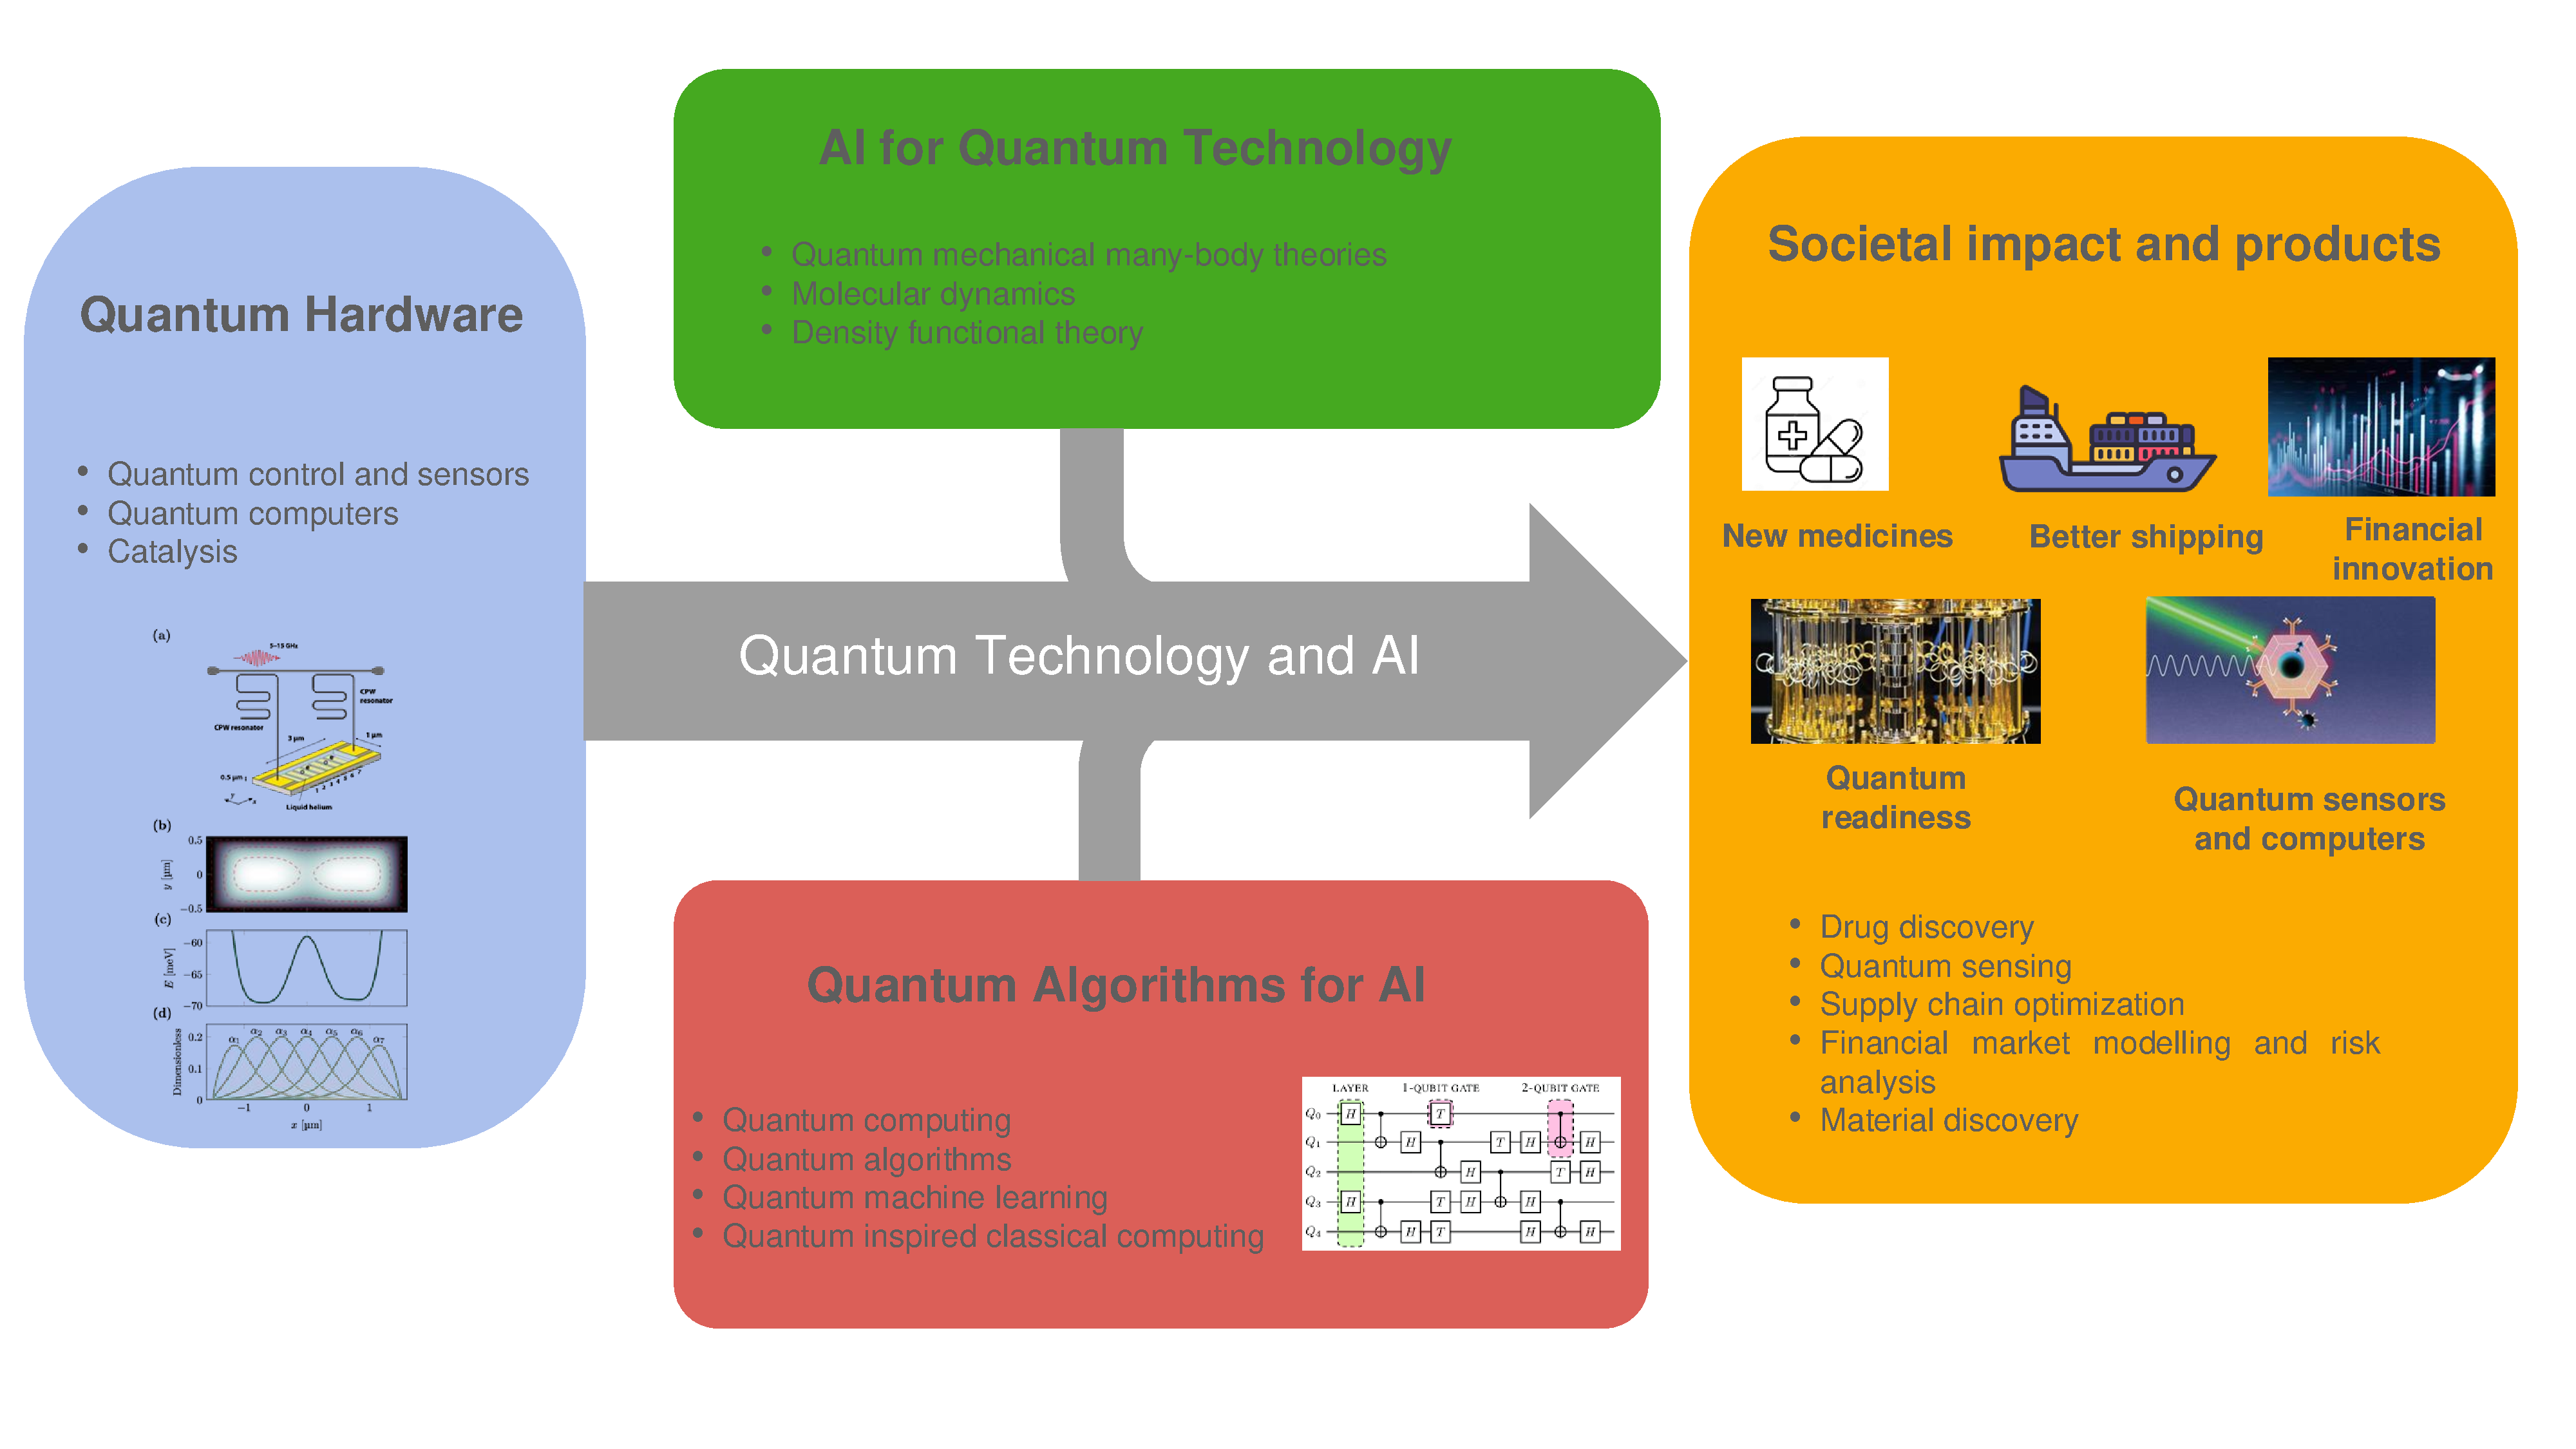
\includegraphics[width=1.05\linewidth]{figures/figureintro.pdf}}

\end{frame}



%-----------------------------------------------------------
\section{Introduction to Machine Learning}
\begin{frame}{What is Machine Learning?}
Machine Learning (ML) is the study of algorithms that improve through data experience.

\textbf{Types of Machine Learning:}
\begin{itemize}
    \item \textbf{Supervised Learning:} Labeled data for classification or regression.
    \item \textbf{Unsupervised Learning:} No labels; discover hidden patterns.
    \item \textbf{Reinforcement Learning:} Learning through interaction with the environment.
\end{itemize}


\textbf{ML Workflow:}
\[
\text{Data} \rightarrow \text{Model Training} \rightarrow \text{Prediction}
\]
\end{frame}



%-----------------------------------------------------------
\section{Introduction to Quantum Computing}
\begin{frame}{What is Quantum Computing?}
Quantum computing leverages principles of quantum mechanics to perform computations beyond classical capabilities.

\vspace{10pt}
\textbf{Key Concepts:}
\begin{itemize}
\item \textbf{Superposition:} Qubits can exist in a combination of states.
\item \textbf{Entanglement:} Correlation between qubits regardless of distance.
\item \textbf{Quantum Interference:} Probability amplitudes interfere to solve problems.
\end{itemize}

\textbf{Qubit Representation:}
\[
\ket{\psi} = \alpha \ket{0} + \beta \ket{1}, \quad |\alpha|^2 + |\beta|^2 = 1
\]
\end{frame}


%-----------------------------------------------------------
\section{Quantum Machine Learning (QML)}
\begin{frame}{What is Quantum Machine Learning?}
\textbf{Quantum Machine Learning (QML)} integrates quantum computing with machine learning algorithms to exploit quantum advantages.

\vspace{10pt}
\textbf{Motivation:}
\begin{itemize}
    \item High-dimensional Hilbert spaces for better feature representation.
    \item Quantum parallelism for faster computation.
    \item Quantum entanglement for richer data encoding.
\end{itemize}


\end{frame}

\section{Quantum Speedups}
\begin{frame}{Quantum Speedups in ML}
\textbf{Why Quantum?}
\begin{itemize}
    \item \textbf{Quantum Parallelism:} Process multiple states simultaneously.
    \item \textbf{Quantum Entanglement:} Correlated states for richer information.
    \item \textbf{Quantum Interference:} Constructive and destructive interference to enhance solutions.
\end{itemize}

\pause
\textbf{Example - Grover's Algorithm:}
\[
\text{Quantum Search Complexity: } O(\sqrt{N}) \text{ vs. } O(N)
\]

\textbf{Advantage:}
- Speedups in high-dimensional optimization and linear algebra problems.
\end{frame}

%-----------------------------------------------------------
\section{Challenges in Quantum Machine Learning}
\begin{frame}{Challenges and Limitations}
\textbf{1. Quantum Hardware Limitations:}
\begin{itemize}
    \item Noisy Intermediate-Scale Quantum (NISQ) devices.
    \item Decoherence and limited qubit coherence times.
\end{itemize}

\textbf{2. Data Encoding:}
\begin{itemize}
    \item Efficient embedding of classical data into quantum states.
\end{itemize}

\textbf{3. Scalability:}
\begin{itemize}
    \item Difficult to scale circuits to large datasets.
\end{itemize}
\end{frame}

%-----------------------------------------------------------
\section{Applications of QML}
\begin{frame}{Applications of Quantum Machine Learning}
\textbf{1. Quantum mechanical many-particle syste,s:}
\begin{itemize}
    \item Simulate molecular structures with QML.
\end{itemize}

\textbf{2. Finance:}
\begin{itemize}
    \item Quantum optimization for portfolio management.
\end{itemize}

\textbf{3. Image Recognition:}
\begin{itemize}
    \item Quantum-enhanced convolutional neural networks.
\end{itemize}
\end{frame}





\begin{frame}[plain,fragile]
\frametitle{AI/ML and some statements you may have heard (and what do they mean?)}



\begin{enumerate}
\item Fei-Fei Li on ImageNet: \textbf{map out the entire world of objects} (\href{{https://cacm.acm.org/news/219702-the-data-that-transformed-ai-research-and-possibly-the-world/fulltext}}{The data that transformed AI research})

\item Russell and Norvig in their popular textbook: \textbf{relevant to any intellectual task; it is truly a universal field} (\href{{http://aima.cs.berkeley.edu/}}{Artificial Intelligence, A modern approach})

\item Woody Bledsoe puts it more bluntly: \textbf{in the long run, AI is the only science} (quoted in Pamilla McCorduck, \href{{https://www.pamelamccorduck.com/machines-who-think}}{Machines who think})
\end{enumerate}

\noindent
If you wish to have a critical read on AI/ML from a societal point of view, see \href{{https://www.katecrawford.net/}}{Kate Crawford's recent text Atlas of AI}.

\textbf{Here: with AI/ML we intend a collection of machine learning methods with an emphasis on statistical learning and data analysis}
\end{frame}






\begin{frame}[plain,fragile]
\frametitle{Machine learning and AI models are computationally expensive}


% inline figure
\centerline{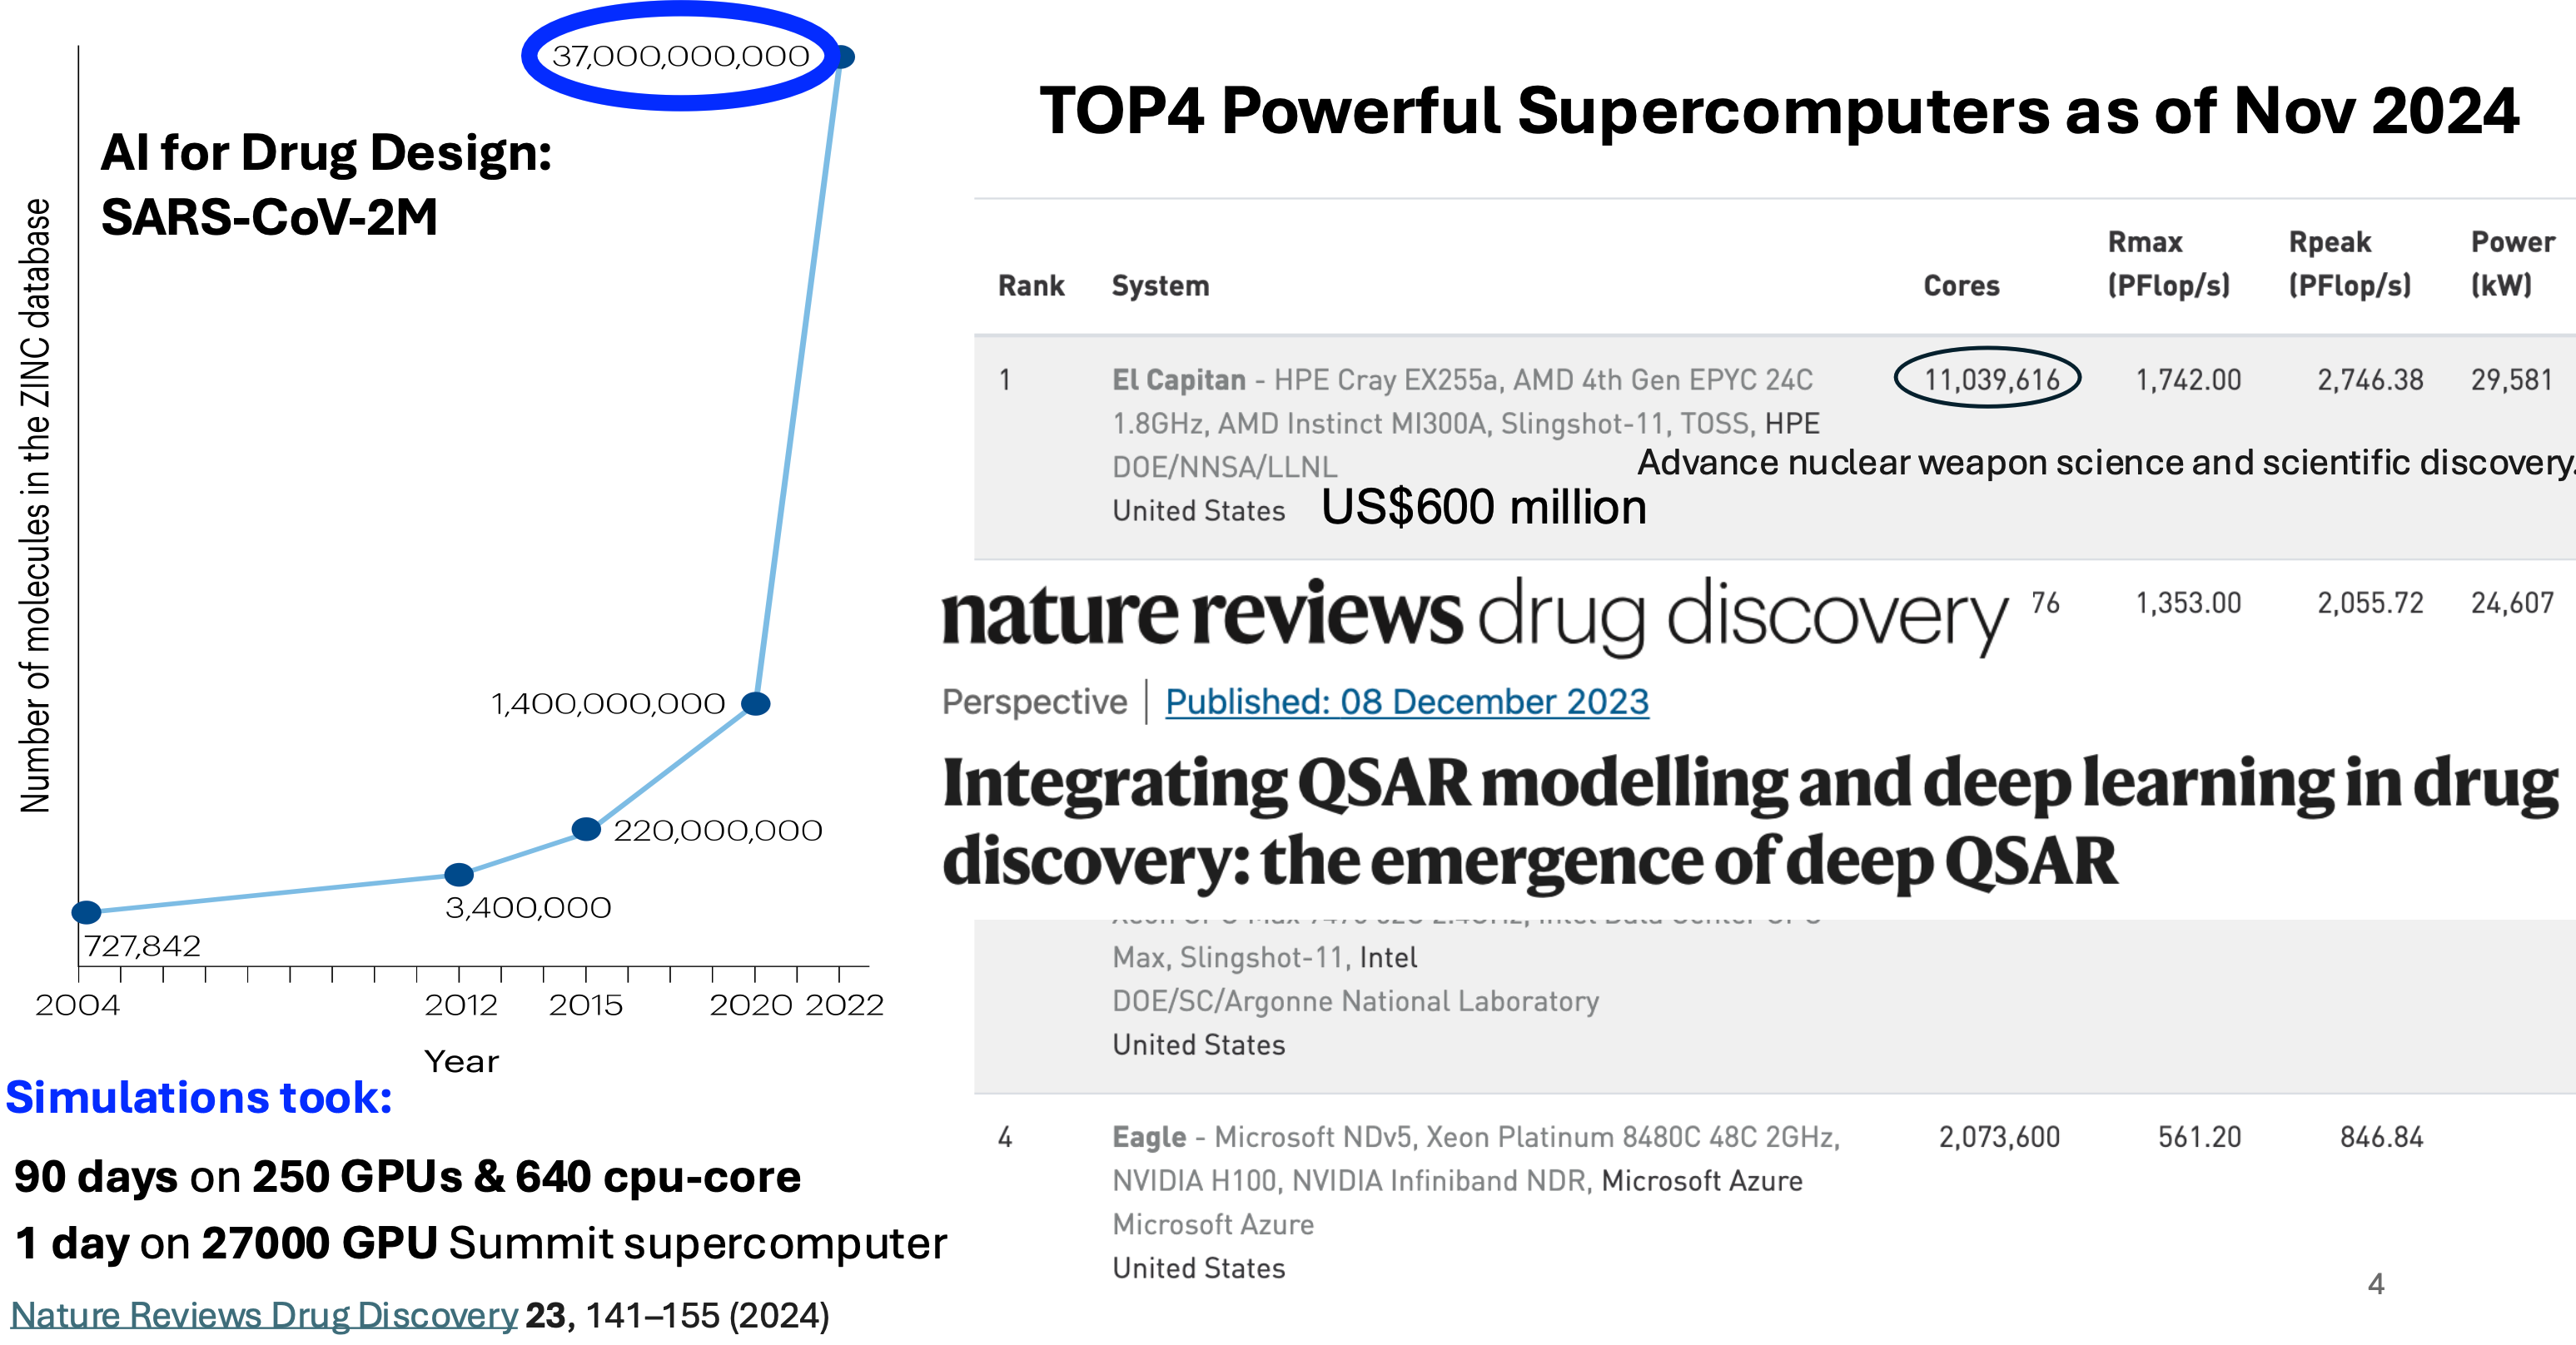
\includegraphics[width=1.0\linewidth]{figures/aitalk2.png}}

\end{frame}


\begin{frame}[plain,fragile]
\frametitle{And power greedy, perhaps quantum computers can reduce the impact?}

% inline figure
\centerline{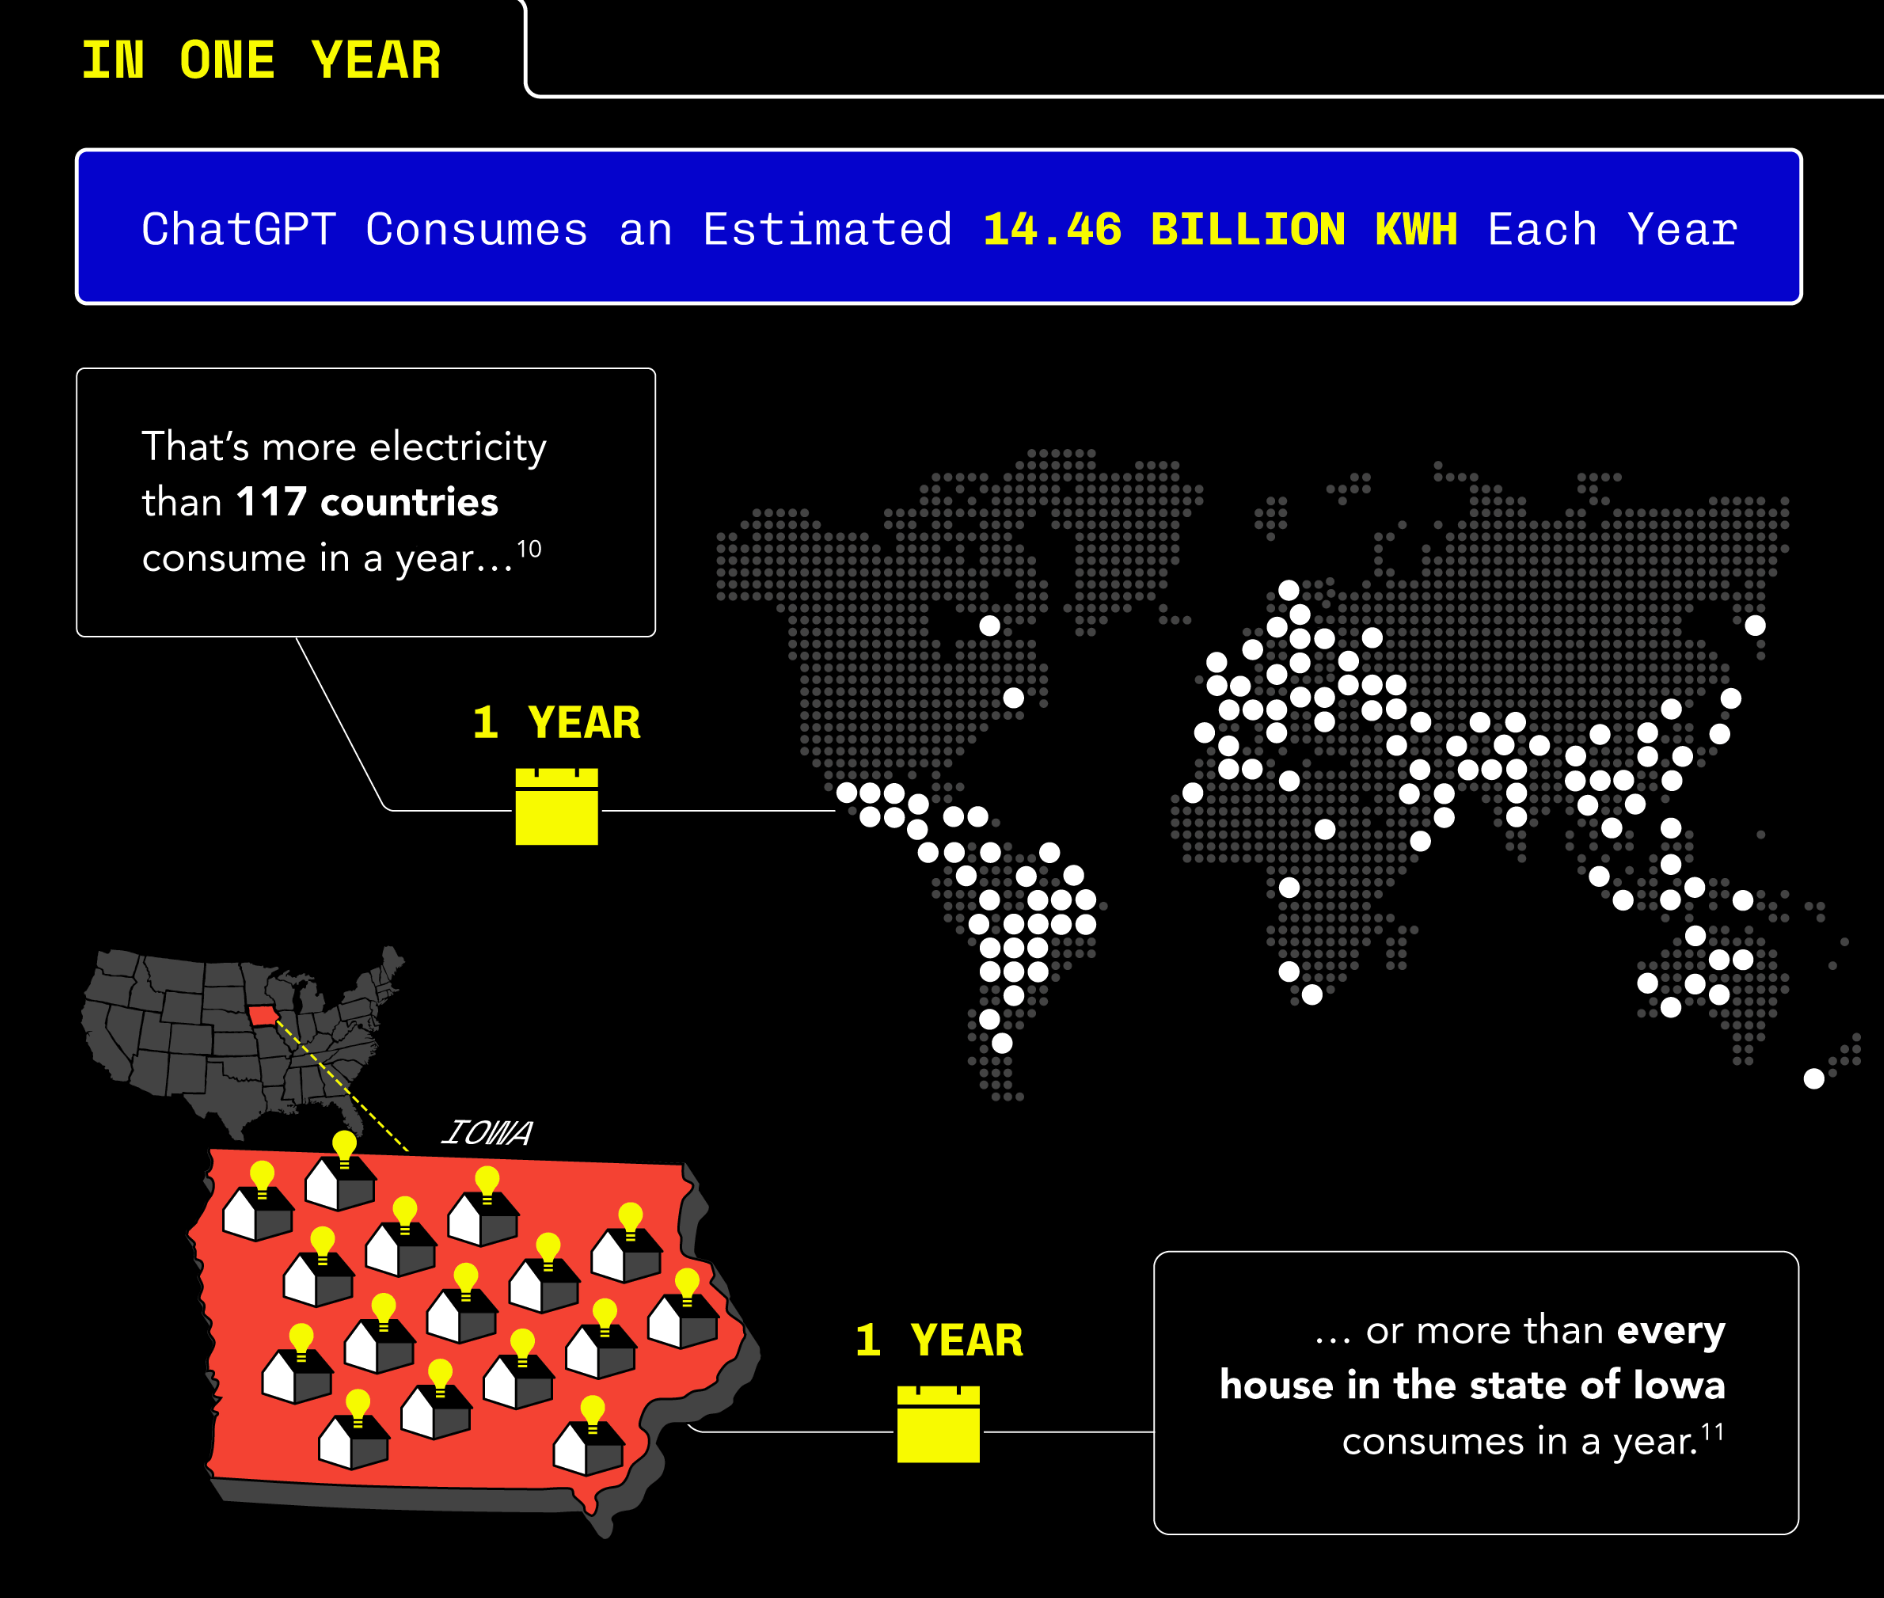
\includegraphics[width=0.7\linewidth]{figures/aitalk1.png}}
Taken from \url{https://www.businessenergyuk.com/knowledge-hub/chatgpt-energy-consumption-visualized/}
\end{frame}



\begin{frame}[plain,fragile]
\frametitle{Main categories of Machine Learning}

\begin{block}{}
Another way to categorize machine learning tasks is to consider the desired output of a system.
Some of the most common tasks are:

\begin{itemize}
  \item Classification: Outputs are divided into two or more classes. The goal is to   produce a model that assigns inputs into one of these classes. An example is to identify  digits based on pictures of hand-written ones. Classification is typically supervised learning.

  \item Regression: Finding a functional relationship between an input data set and a reference data set.   The goal is to construct a function that maps input data to continuous output values.

  \item Clustering: Data are divided into groups with certain common traits, without knowing the different groups beforehand.  It is thus a form of unsupervised learning.
\end{itemize}

\noindent
\end{block}
\end{frame}





\begin{frame}[plain,fragile]
\frametitle{The plethora  of machine learning algorithms/methods}

\begin{enumerate}
\item Deep learning: Neural Networks (NN), Convolutional NN, Recurrent NN, Boltzmann machines, autoencoders and variational autoencoders  and generative adversarial networks, stable diffusion and many more generative models

\item Bayesian statistics and Bayesian Machine Learning, Bayesian experimental design, Bayesian Regression models, Bayesian neural networks, Gaussian processes and much more

\item Dimensionality reduction (Principal component analysis), Clustering Methods and more

\item Ensemble Methods, Random forests, bagging and voting methods, gradient boosting approaches 

\item Linear and logistic regression, Kernel methods, support vector machines and more

\item Reinforcement Learning; Transfer Learning and more 
\end{enumerate}

\noindent
\end{frame}





\begin{frame}[plain,fragile]
\frametitle{Example of discriminative modeling, \href{{https://www.oreilly.com/library/view/generative-deep-learning/9781098134174/ch01.html}}{taken from Generative Deep Learning by David Foster}}

\vspace{6mm}

% inline figure
\centerline{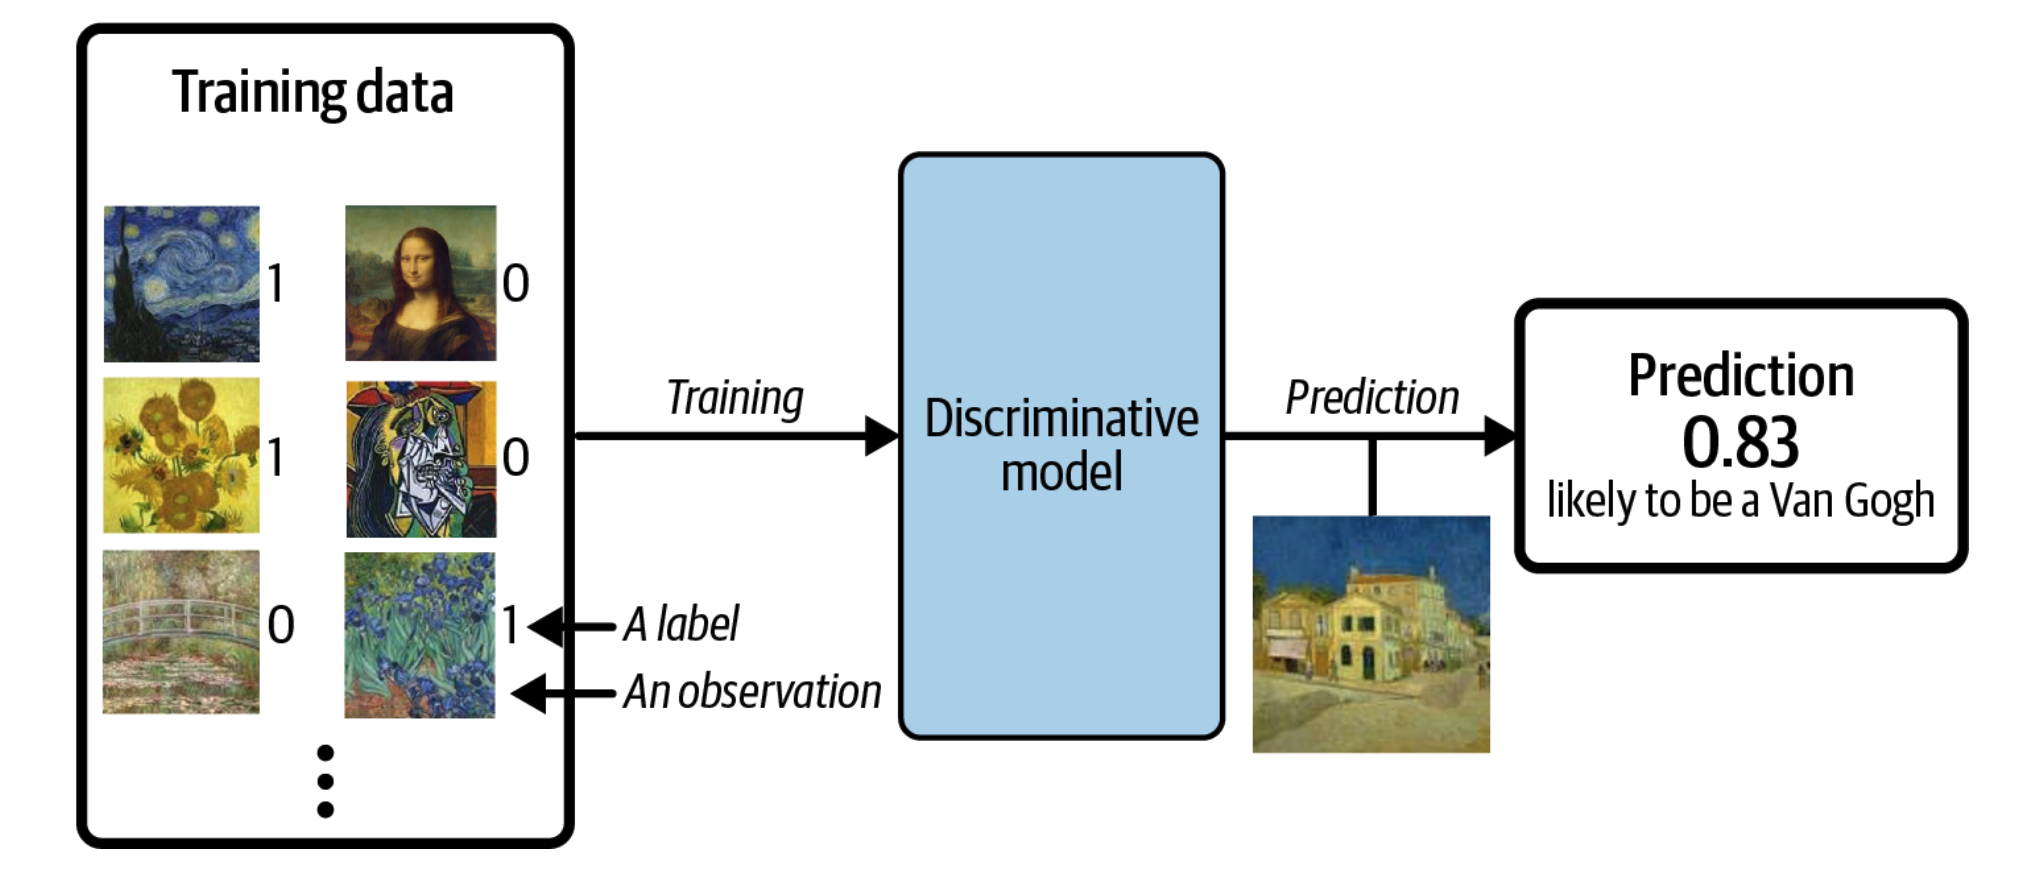
\includegraphics[width=1.0\linewidth]{figures/standarddeeplearning.png}}

\vspace{6mm}
\end{frame}

\begin{frame}[plain,fragile]
\frametitle{Example of generative modeling, \href{{https://www.oreilly.com/library/view/generative-deep-learning/9781098134174/ch01.html}}{taken from Generative Deep Learning by David Foster}}

\vspace{6mm}

% inline figure
\centerline{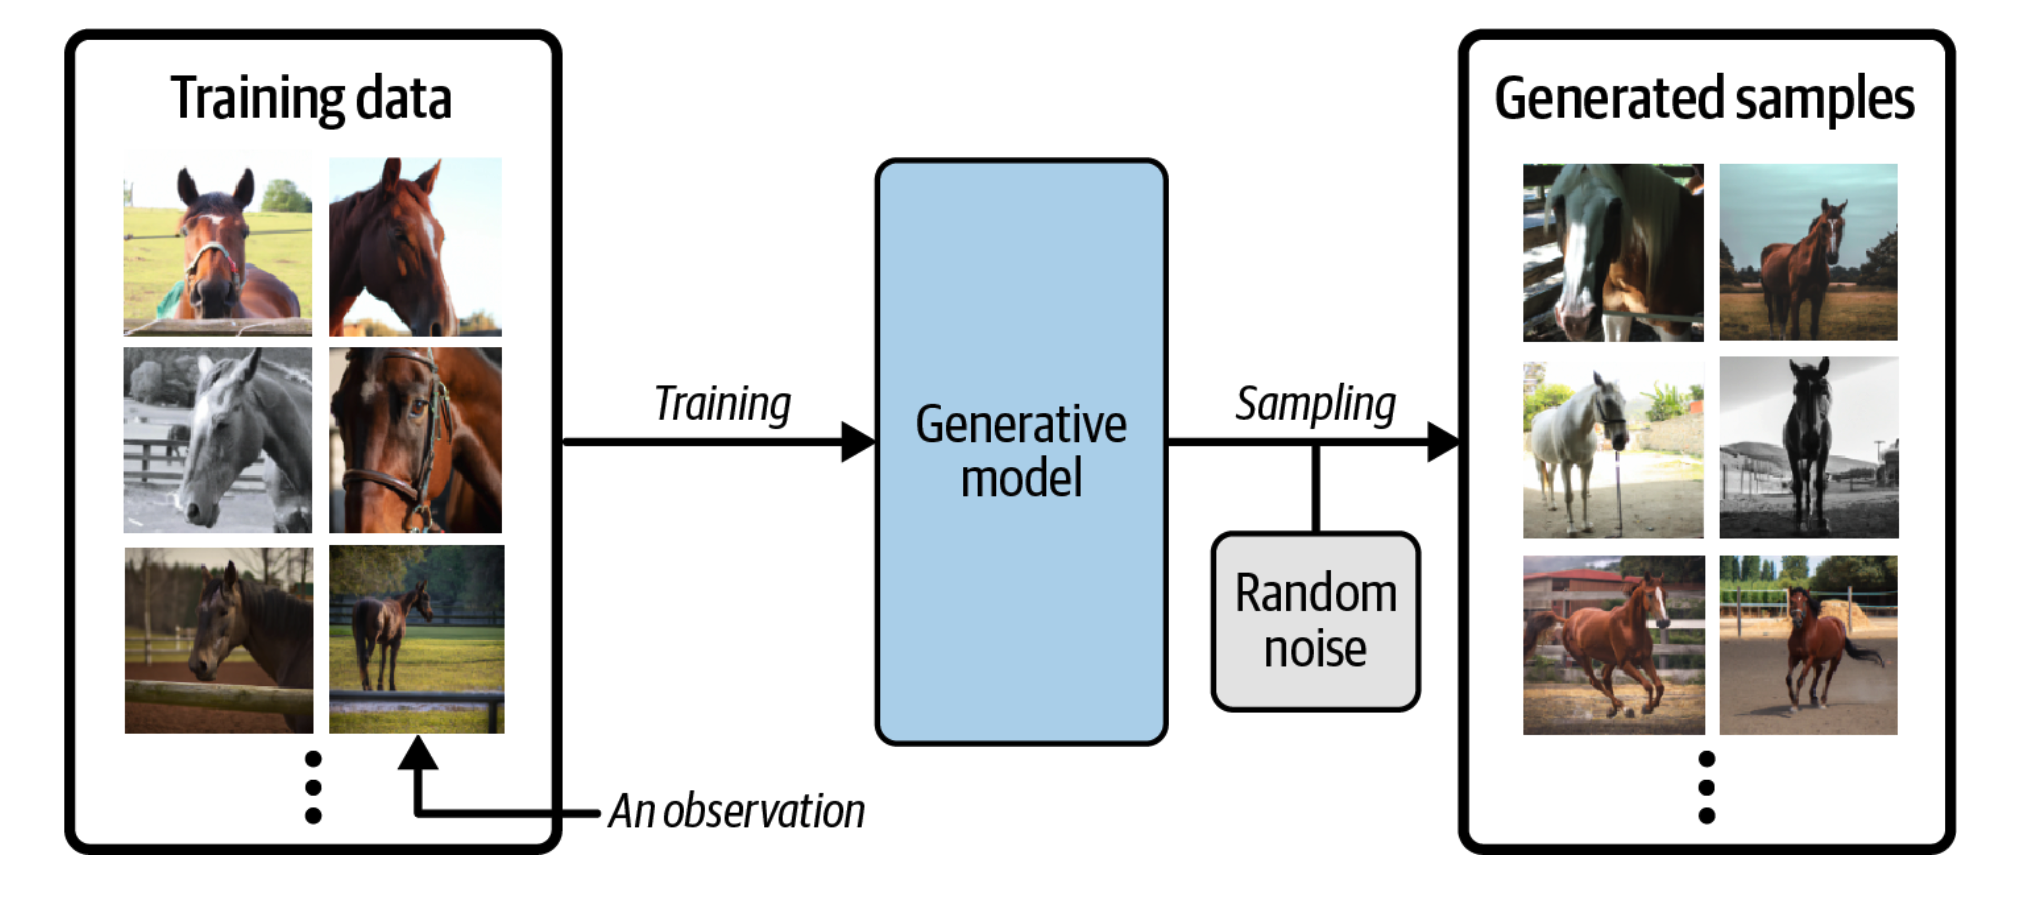
\includegraphics[width=1.0\linewidth]{figures/generativelearning.png}}

\vspace{6mm}
\end{frame}

\begin{frame}[plain,fragile]
\frametitle{Taxonomy of generative deep learning, \href{{https://www.oreilly.com/library/view/generative-deep-learning/9781098134174/ch01.html}}{taken from Generative Deep Learning by David Foster}}

\vspace{6mm}

% inline figure
\centerline{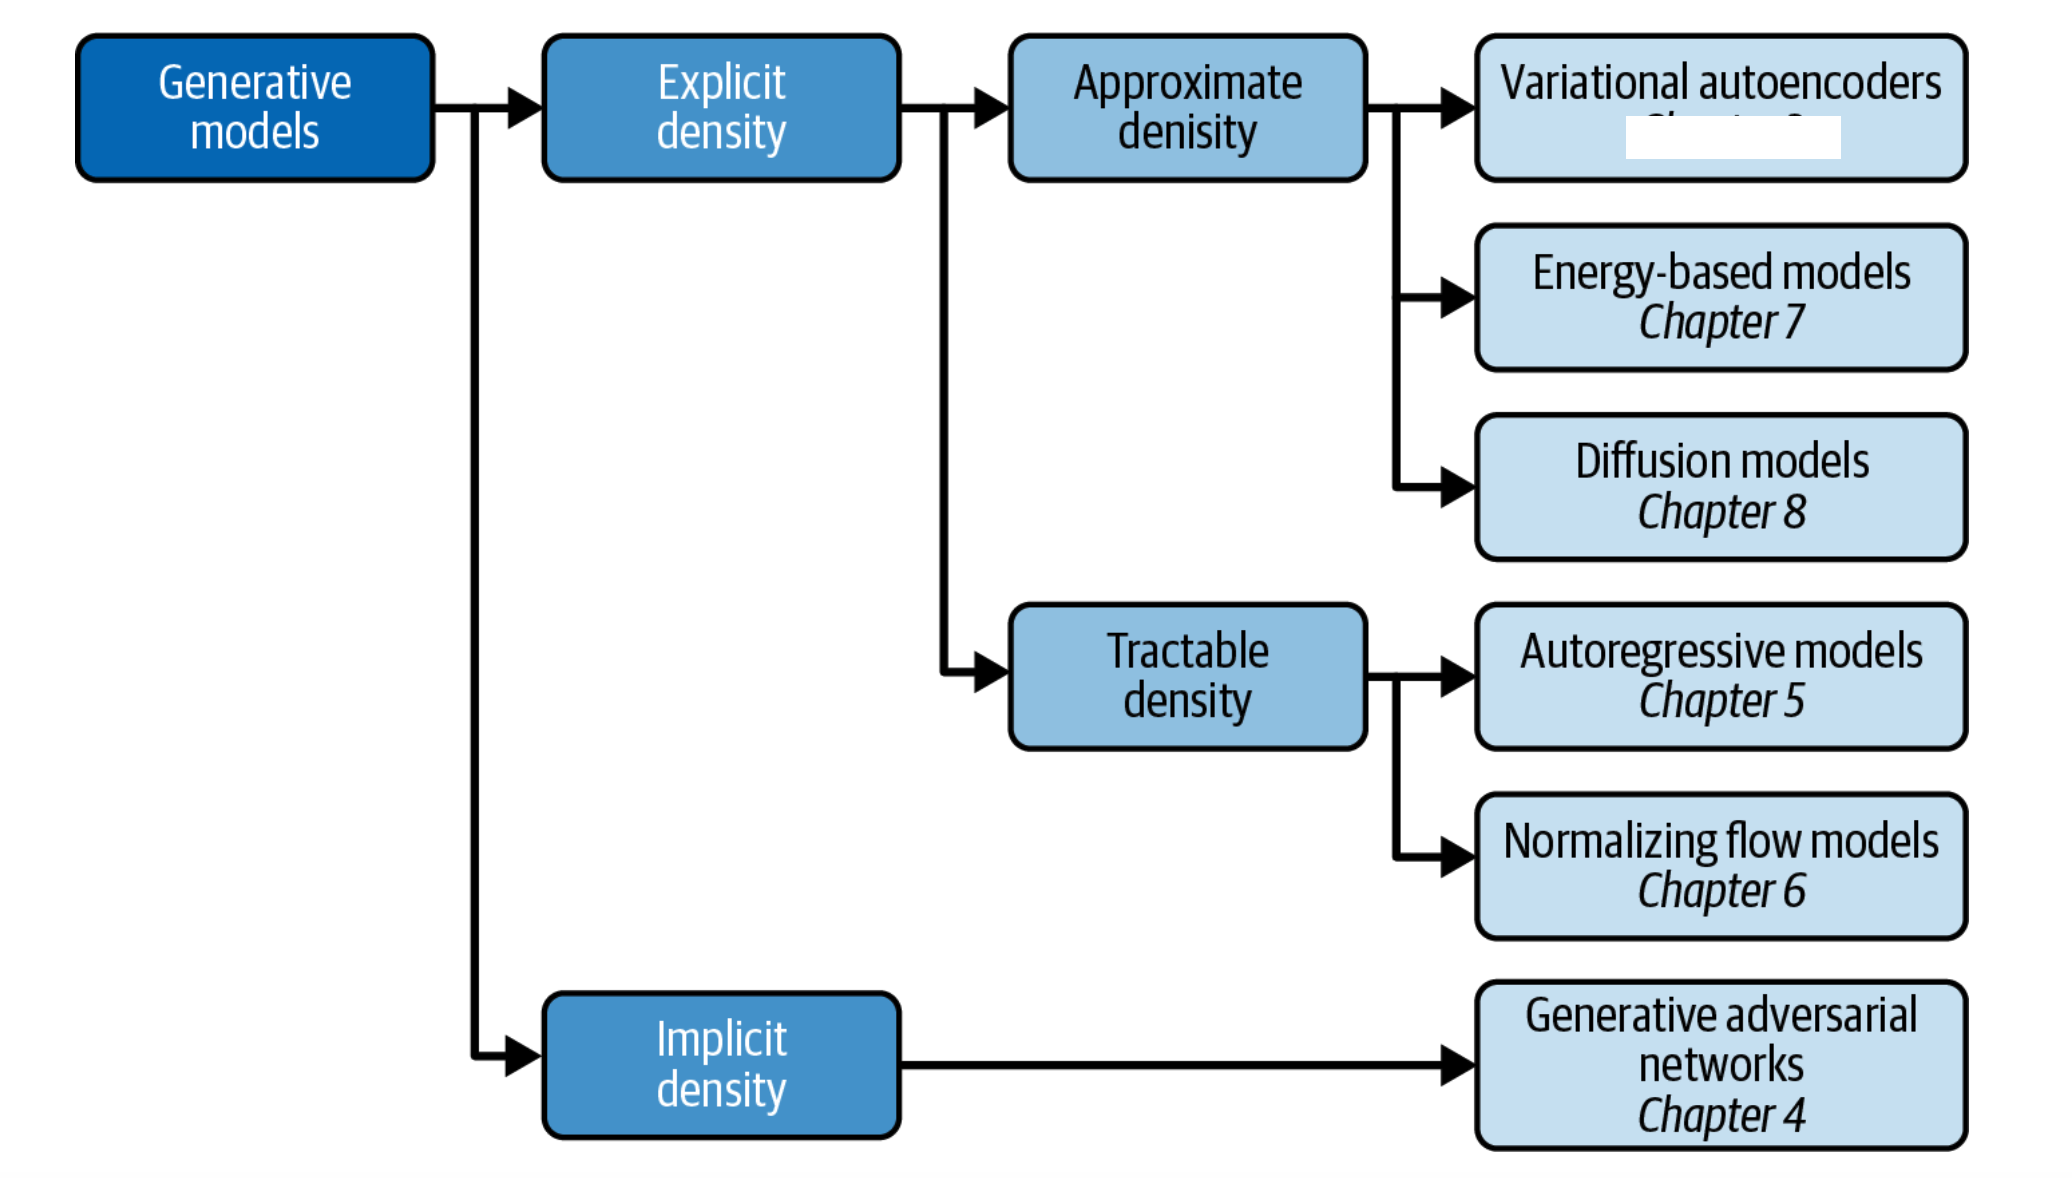
\includegraphics[width=1.0\linewidth]{figures/generativemodels.png}}

\vspace{6mm}
\end{frame}


\begin{frame}[plain,fragile]
\frametitle{What are the basic Machine Learning ingredients?}

\begin{block}{}
Almost every problem in ML and data science starts with the same ingredients:
\begin{itemize}
\item The dataset $\bm{x}$ (could be some observable quantity of the system we are studying)

\item A model which is a function of a set of parameters $\bm{\alpha}$ that relates to the dataset, say a likelihood  function $p(\bm{x}\vert \bm{\alpha})$ or just a simple model $f(\bm{\alpha})$

\item A so-called \textbf{loss/cost/risk} function $\mathcal{C} (\bm{x}, f(\bm{\alpha}))$ which allows us to decide how well our model represents the dataset. 
\end{itemize}

\noindent
We seek to minimize the function $\mathcal{C} (\bm{x}, f(\bm{\alpha}))$ by finding the parameter values which minimize $\mathcal{C}$. This leads to  various minimization algorithms. It may surprise many, but at the heart of all machine learning algortihms there is an optimization problem. 
\end{block}
\end{frame}

\begin{frame}[plain,fragile]
\frametitle{Low-level machine learning, the family of ordinary least squares methods}

Our data which we want to apply a machine learning method on, consist
of a set of inputs $\bm{x}^T=[x_0,x_1,x_2,\dots,x_{n-1}]$ and the
outputs we want to model $\bm{y}^T=[y_0,y_1,y_2,\dots,y_{n-1}]$.
We assume  that the output data can be represented (for a regression case) by a continuous function $f$
through
\[
\bm{y}=f(\bm{x})+\bm{\epsilon}.
\]
\end{frame}

\begin{frame}[plain,fragile]
\frametitle{Setting up the equations}

In linear regression we approximate the unknown function with another
continuous function $\tilde{\bm{y}}(\bm{x})$ which depends linearly on
some unknown parameters
$\bm{\theta}^T=[\theta_0,\theta_1,\theta_2,\dots,\theta_{p-1}]$.

The input data can be organized in terms of a so-called design matrix 
with an approximating function $\bm{\tilde{y}}$ 
\[
\bm{\tilde{y}}= \bm{X}\bm{\theta},
\]
\end{frame}

\begin{frame}[plain,fragile]
\frametitle{The objective/cost/loss function}

The  simplest approach is the mean squared error
\[
C(\bm{\Theta})=\frac{1}{n}\sum_{i=0}^{n-1}\left(y_i-\tilde{y}_i\right)^2=\frac{1}{n}\left\{\left(\bm{y}-\bm{\tilde{y}}\right)^T\left(\bm{y}-\bm{\tilde{y}}\right)\right\},
\]
or using the matrix $\bm{X}$ and in a more compact matrix-vector notation as
\[
C(\bm{\Theta})=\frac{1}{n}\left\{\left(\bm{y}-\bm{X}\bm{\theta}\right)^T\left(\bm{y}-\bm{X}\bm{\theta}\right)\right\}.
\]
This function represents one of many possible ways to define the so-called cost function.
\end{frame}

\begin{frame}[plain,fragile]
\frametitle{Training solution}

Optimizing with respect to the unknown parameters $\theta_j$ we get 
\[
\bm{X}^T\bm{y} = \bm{X}^T\bm{X}\bm{\theta},  
\]
and if the matrix $\bm{X}^T\bm{X}$ is invertible we have the optimal values
\[
\hat{\bm{\theta}} =\left(\bm{X}^T\bm{X}\right)^{-1}\bm{X}^T\bm{y}.
\]

We say we 'learn' the unknown parameters $\bm{\theta}$ from the last equation.
\end{frame}


\begin{frame}[plain,fragile]
\frametitle{Schematic view on Machine Learning approaches}


% inline figure
\centerline{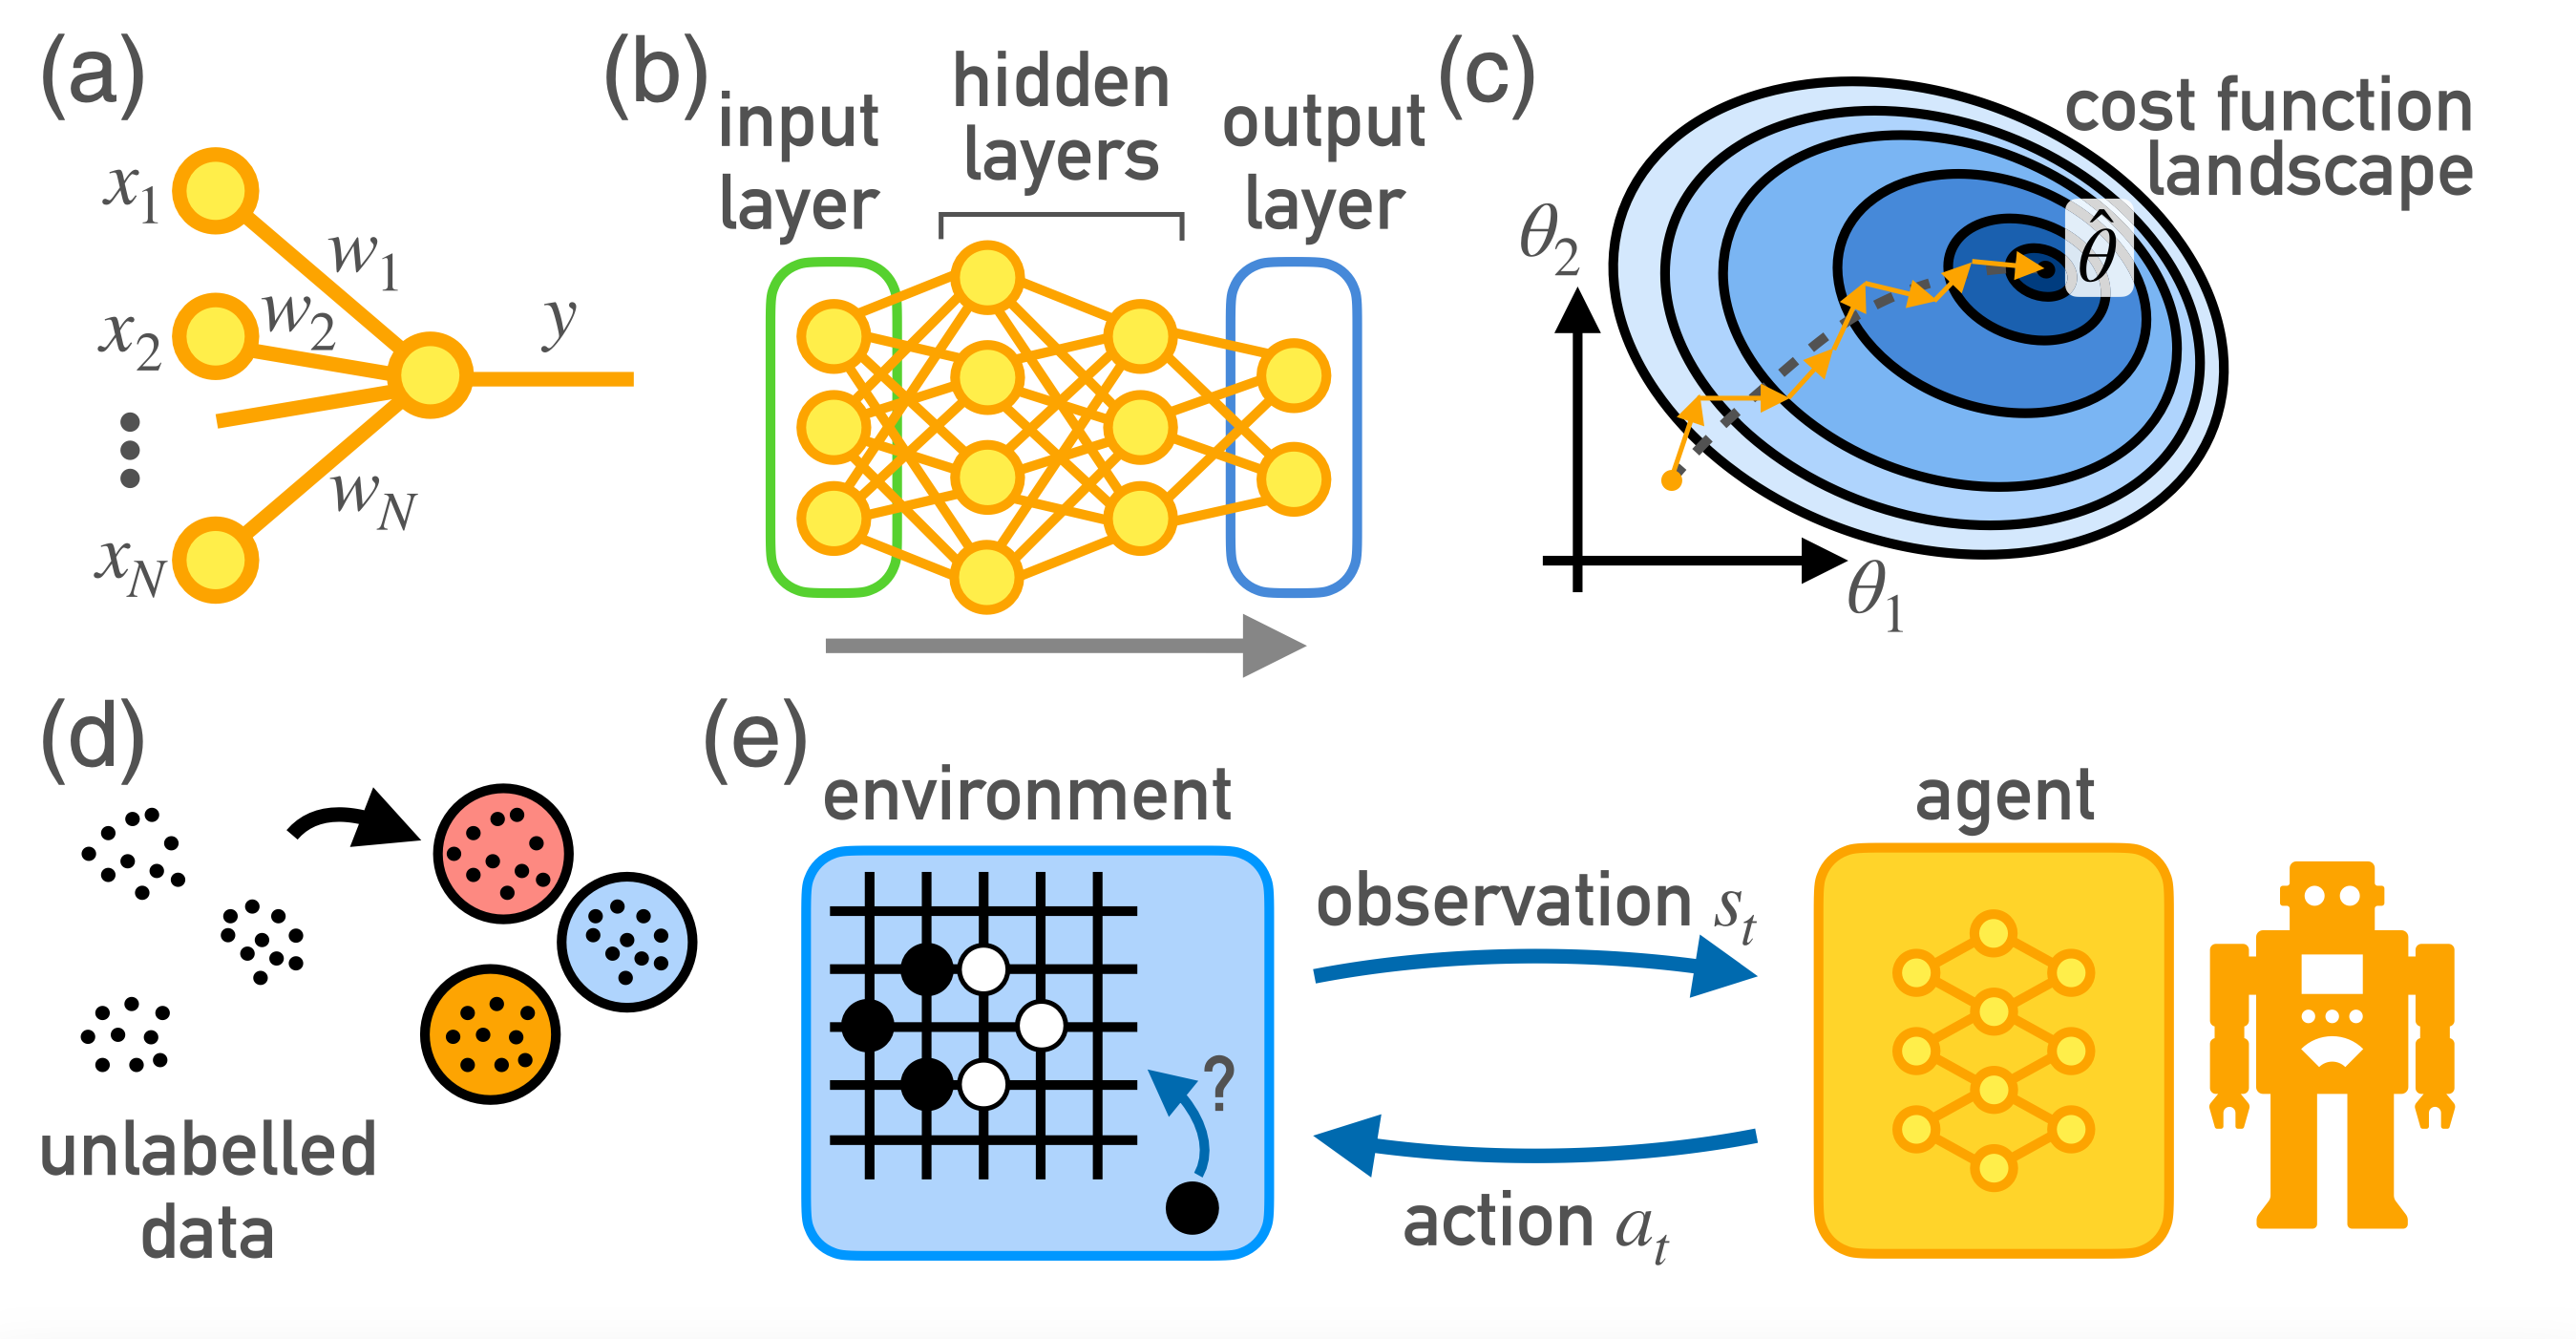
\includegraphics[width=1.05\linewidth]{figures/krenn2}}

\end{frame}




\begin{frame}[plain,fragile]
\frametitle{Scientific Machine Learning}

An important and emerging field is what has been dubbed as scientific ML, see the article by Deiana et al, Applications and Techniques for Fast Machine Learning in Science, Big Data \textbf{5}, 787421 (2022) \href{{https://doi.org/10.3389/fdata.2022.787421}}{\nolinkurl{https://doi.org/10.3389/fdata.2022.787421}}

\begin{block}{}
The authors discuss applications and techniques for fast machine
learning (ML) in science -- the concept of integrating power ML
methods into the real-time experimental data processing loop to
accelerate scientific discovery. The report covers three main areas

\begin{enumerate}
\item applications for fast ML across a number of scientific domains;

\item techniques for training and implementing performant and resource-efficient ML algorithms;

\item and computing architectures, platforms, and technologies for deploying these algorithms.
\end{enumerate}

\noindent
\end{block}
\end{frame}

\begin{frame}[plain,fragile]
\frametitle{ML for detectors}

\vspace{6mm}

% inline figure
\centerline{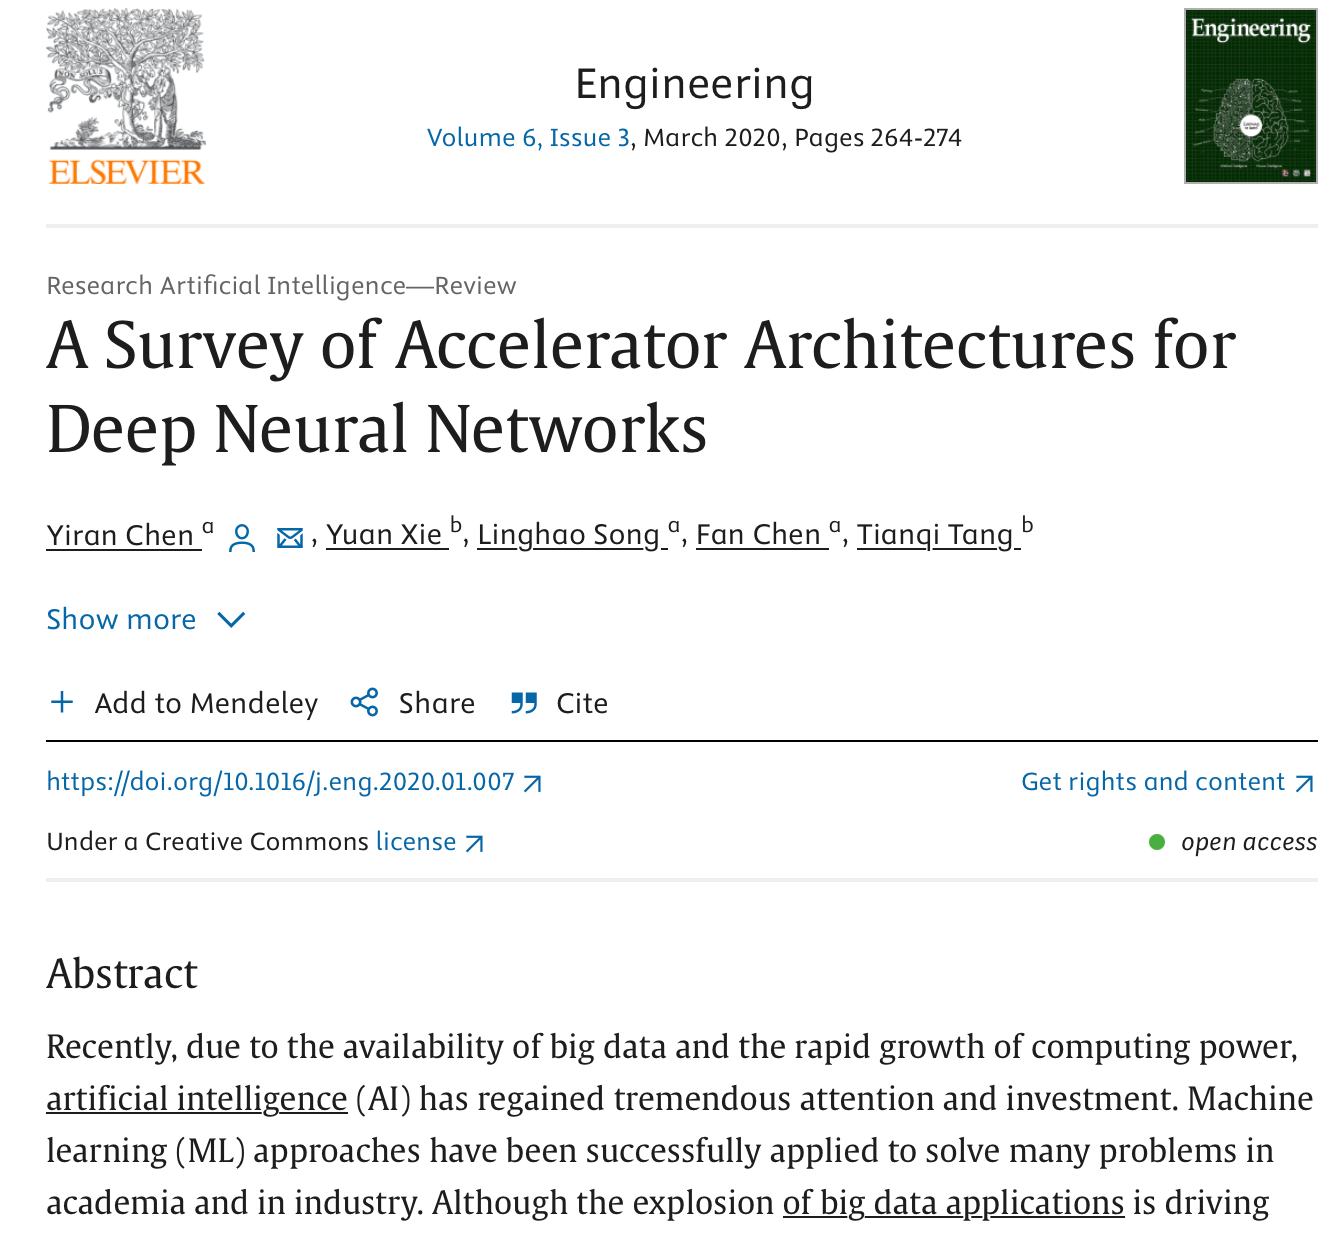
\includegraphics[width=1.0\linewidth]{figures/detectors.png}}

\vspace{6mm}
\end{frame}


\begin{frame}[plain,fragile]
\frametitle{Physics driven Machine Learning}

Another hot topic is what has loosely been dubbed \textbf{Physics-driven deep learning}. See the recent work on \href{{https://www.nature.com/articles/s42256-021-00302-5}}{Learning nonlinear operators via DeepONet based on the universal approximation theorem of operators, Nature Machine Learning, vol 3, 218 (2021)}.

\end{frame}

\begin{frame}[plain,fragile]
\frametitle{And more}

\begin{block}{}
\begin{itemize}
\item An important application of AI/ML methods is to improve the estimation of bias or uncertainty due to the introduction of or lack of physical constraints in various theoretical models.

\item We expect to use AI/ML algorithms and methods to improve our knowledge about  correlations of physical model parameters in data for complex systems. Deep learning methods show great promise in circumventing the exploding dimensionalities encountered in many problems.

\end{itemize}

\noindent
\end{block}
\end{frame}

\begin{frame}[plain,fragile]
\frametitle{Argon-46 by Solli et al., NIMA 1010, 165461 (2021)}

\begin{block}{}
Each row is one event in two projections,
where the color intensity of each point indicates higher charge values
recorded by the detector. The bottom row illustrates a carbon event with
a large fraction of noise, while the top row shows a proton event
almost free of noise. 
\end{block}

% inline figure
\centerline{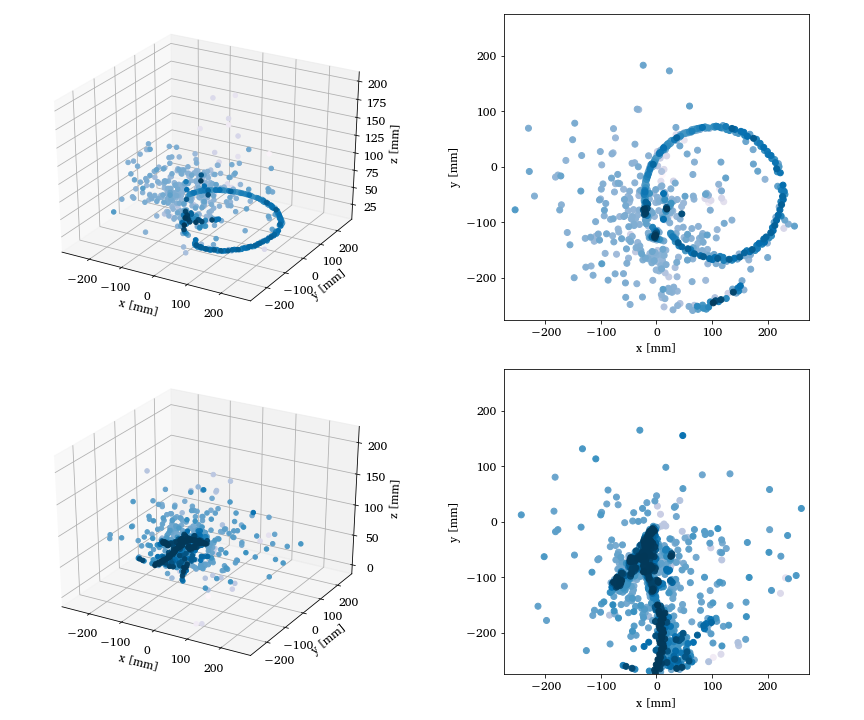
\includegraphics[width=0.6\linewidth]{figures/examples_raw.png}}

\vspace{6mm}
\end{frame}

\begin{frame}[plain,fragile]
\frametitle{Many-body physics, Quantum Monte Carlo and deep learning}

\begin{block}{}
Given a hamiltonian $H$ and a trial wave function $\Psi_T$, the variational principle states that the expectation value of $\langle H \rangle$, defined through 
\[
   \langle E \rangle =
   \frac{\int d\bm{R}\Psi^{\ast}_T(\bm{R})H(\bm{R})\Psi_T(\bm{R})}
        {\int d\bm{R}\Psi^{\ast}_T(\bm{R})\Psi_T(\bm{R})},
\]
is an upper bound to the ground state energy $E_0$ of the hamiltonian $H$, that is 
\[
    E_0 \le \langle E \rangle.
\]
In general, the integrals involved in the calculation of various  expectation values  are multi-dimensional ones. Traditional integration methods such as the Gauss-Legendre will not be adequate for say the  computation of the energy of a many-body system.  \textbf{Basic philosophy: Let a neural network find the optimal wave function}
\end{block}
\end{frame}

\begin{frame}[plain,fragile]
\frametitle{Why Feed Forward Neural Networks (FFNN)?}

According to the \emph{Universal approximation theorem}, a feed-forward
neural network with just a single hidden layer containing a finite
number of neurons can approximate a continuous multidimensional
function to arbitrary accuracy, assuming the activation function for
the hidden layer is a \textbf{non-constant, bounded and
monotonically-increasing continuous function}.
\end{frame}



\begin{frame}[plain,fragile]
\frametitle{\href{{https://journals.aps.org/prresearch/pdf/10.1103/PhysRevResearch.5.033062}}{Dilute neutron star matter from neural-network quantum states by Fore et al, Physical Review Research 5, 033062 (2023)} at density $\rho=0.04$ fm$^{-3}$}

\centerline{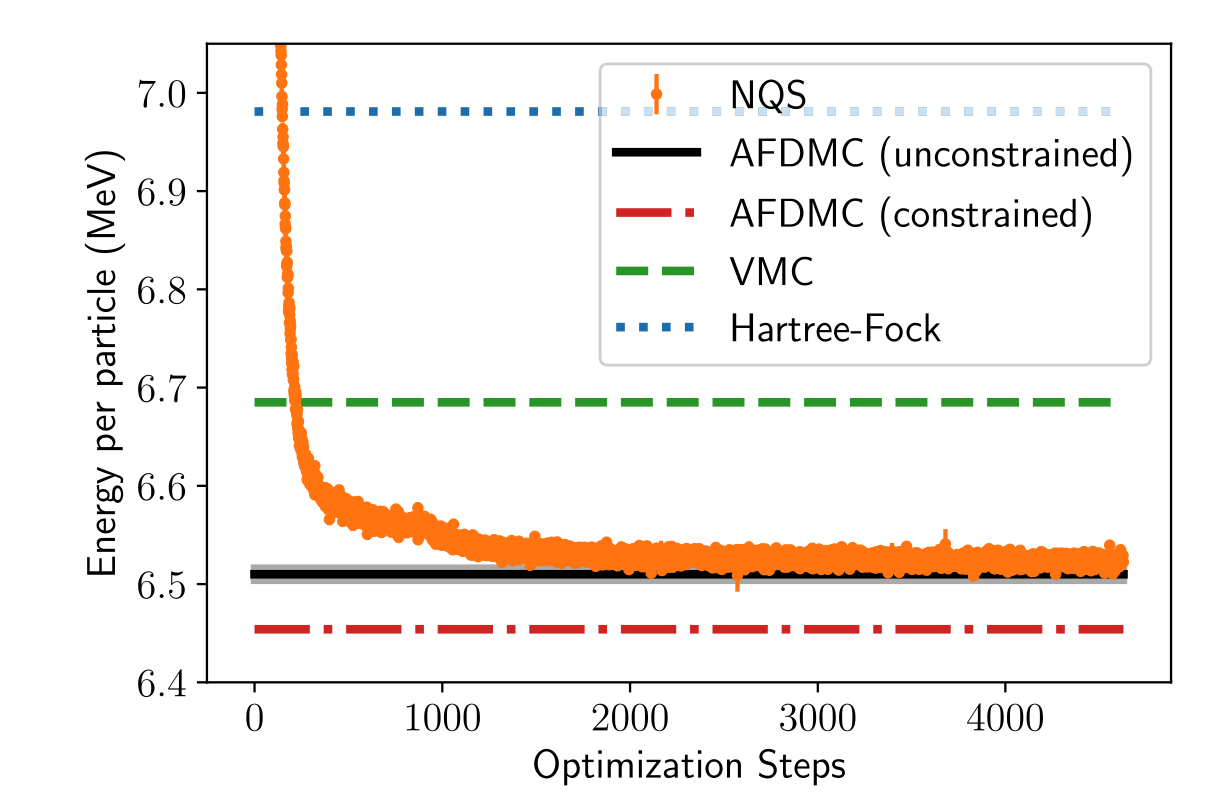
\includegraphics[width=0.9\linewidth]{figures/nmatter.png}}

\end{frame}



\begin{frame}[plain,fragile]
\frametitle{And then quantum engineering}


% inline figure
\centerline{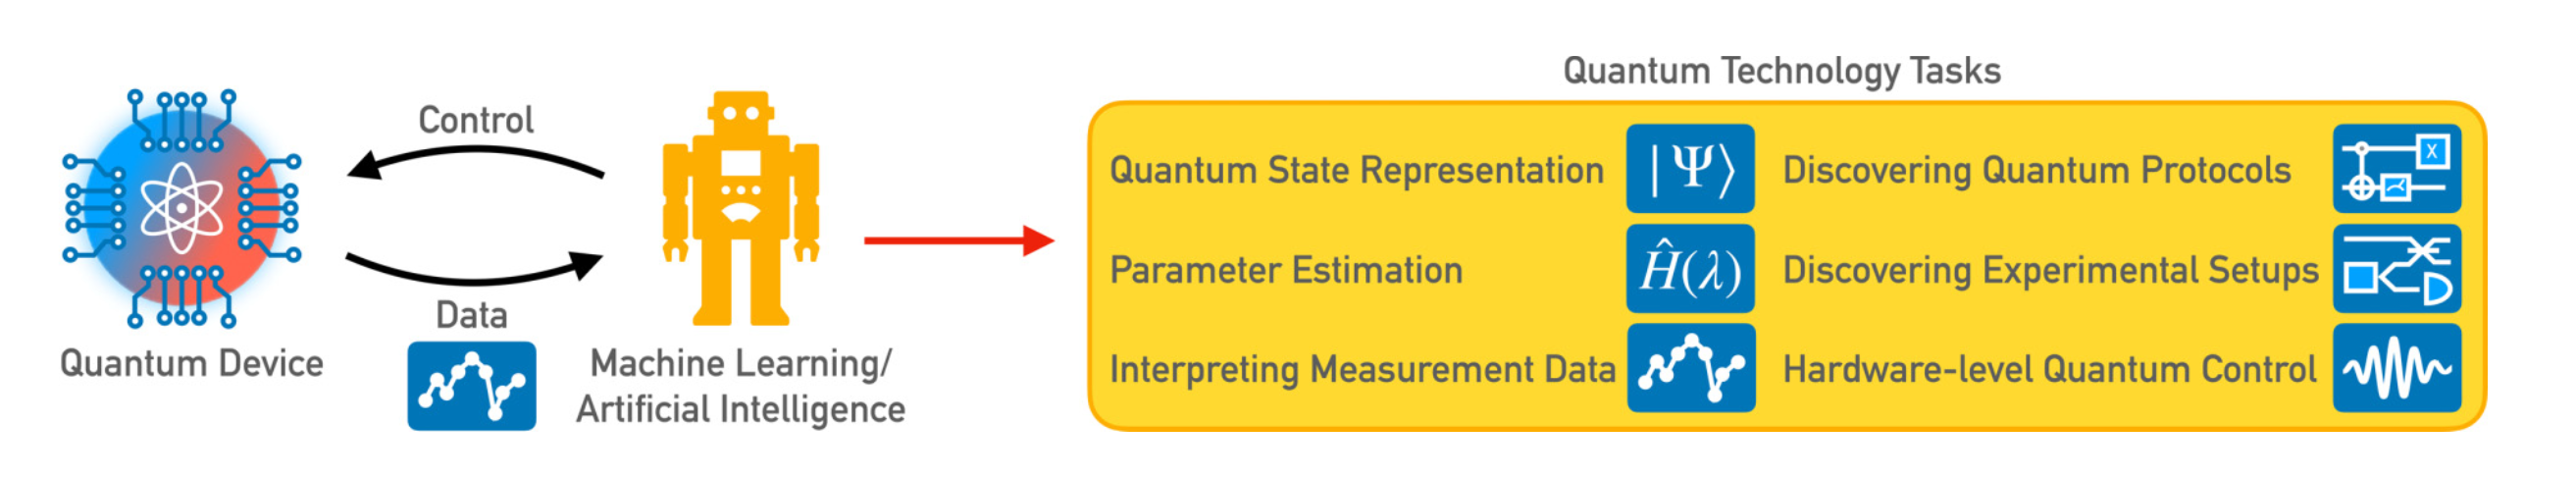
\includegraphics[width=1.05\linewidth]{figures/krenn1}}

\end{frame}






\section{Additional material}





%-----------------------------------------------------------
\section{Quantum Algorithms for ML}
\begin{frame}{1. Quantum Support Vector Machines (QSVM)}
\textbf{Quantum Kernel Estimation:}
\begin{itemize}
    \item Maps classical data to a quantum Hilbert space.
    \item Quantum kernel measures similarity in high-dimensional space.
\end{itemize}

\pause
\textbf{Quantum Kernel:}
\[
K(x, x') = |\braket{\psi(x) | \psi(x')}|^2
\]

\textbf{Advantage:}
- Potentially exponential speedup over classical SVMs.
\end{frame}

%-----------------------------------------------------------
\begin{frame}{2. Quantum Neural Networks (QNNs)}
\textbf{Quantum Neural Networks} replace classical neurons with parameterized quantum circuits.

\textbf{Key Concepts:}
\begin{itemize}
    \item Quantum Gates as Activation Functions.
    \item Variational Quantum Circuits (VQCs) for optimization.
\end{itemize}

\pause
\textbf{Parameterized Quantum Circuit:}
\[
U(\theta) = \prod_i R_y(\theta_i) \cdot CNOT \cdot R_x(\theta_i)
\]

\textbf{Advantage:}
- Quantum gradients enable exploration of non-convex landscapes.
\end{frame}

%-----------------------------------------------------------
\begin{frame}{3. Quantum Boltzmann Machines (QBMs)}
\textbf{Quantum Boltzmann Machines} leverage quantum mechanics to sample from a probability distribution.

\begin{itemize}
    \item Quantum tunneling aids in escaping local minima.
    \item Quantum annealing for optimization problems.
\end{itemize}

\pause
\textbf{Quantum Hamiltonian:}
\[
H = -\sum_i b_i \sigma_i^z - \sum_{ij} w_{ij} \sigma_i^z \sigma_j^z
\]

\textbf{Advantage:}
- Efficient sampling in complex probability distributions.
\end{frame}

%-----------------------------------------------------------
%-----------------------------------------------------------
\section{Future Perspectives}
\begin{frame}{Future Perspectives in QML}
\textbf{1. Fault-Tolerant Quantum Computing:}
\begin{itemize}
    \item Overcoming noise for stable quantum circuits.
\end{itemize}

\textbf{2. Hybrid Quantum-Classical Models:}
\begin{itemize}
    \item Combining quantum circuits with classical neural networks.
\end{itemize}

\textbf{3. Quantum Internet:}
\begin{itemize}
    \item Distributed quantum machine learning over quantum networks.
\end{itemize}
\end{frame}



\begin{frame}[plain,fragile]
\frametitle{Observations (or conclusions if you prefer)}


\begin{block}{}
\begin{itemize}
\item How do we develop insights, competences, knowledge in statistical learning that can advance a given field?
\begin{itemize}

  \item For example: Can we use ML to find out which correlations are relevant and thereby diminish the dimensionality problem in standard many-body  theories?

  \item Can we use AI/ML in detector analysis, accelerator design, analysis of experimental data and more?

  \item Can we use AL/ML to carry out reliable extrapolations by using current experimental knowledge and current theoretical models?

\end{itemize}

\noindent
\item The community needs to invest in relevant educational efforts and training of scientists with knowledge in AI/ML. These are great challenges to the CS and DS communities

\item Quantum computing and quantum machine learning not discussed here

\item Most likely tons of things I have forgotten
\end{itemize}

\noindent
\end{block}
\end{frame}



\end{document}









\begin{frame}[plain,fragile]
\frametitle{Universal approximation theorem}

The universal approximation theorem plays a central role in deep
learning.  \href{{https://link.springer.com/article/10.1007/BF02551274}}{Cybenko (1989)} showed
the following:

\begin{block}{}
Let $\sigma$ be any continuous sigmoidal function such that
\[
\sigma(z) = \left\{\begin{array}{cc} 1 & z\rightarrow \infty\\ 0 & z \rightarrow -\infty \end{array}\right.
\]
Given a continuous and deterministic function $F(\bm{x})$ on the unit
cube in $d$-dimensions $F\in [0,1]^d$, $x\in [0,1]^d$ and a parameter
$\epsilon >0$, there is a one-layer (hidden) neural network
$f(\bm{x};\bm{\Theta})$ with $\bm{\Theta}=(\bm{W},\bm{b})$ and $\bm{W}\in
\mathbb{R}^{m\times n}$ and $\bm{b}\in \mathbb{R}^{n}$, for which
\[
\vert F(\bm{x})-f(\bm{x};\bm{\Theta})\vert < \epsilon \hspace{0.1cm} \forall \bm{x}\in[0,1]^d.
\]

\end{block}
\end{frame}

\begin{frame}[plain,fragile]
\frametitle{The approximation theorem in words}

\textbf{Any continuous function $y=F(\bm{x})$ supported on the unit cube in
$d$-dimensions can be approximated by a one-layer sigmoidal network to
arbitrary accuracy.}

\href{{https://www.sciencedirect.com/science/article/abs/pii/089360809190009T}}{Hornik (1991)} extended the theorem by letting any non-constant, bounded activation function to be included using that the expectation value
\[
\mathbb{E}[\vert F(\bm{x})\vert^2] =\int_{\bm{x}\in D} \vert F(\bm{x})\vert^2p(\bm{x})d\bm{x} < \infty.
\]
Then we have
\[
\mathbb{E}[\vert F(\bm{x})-f(\bm{x};\bm{\Theta})\vert^2] =\int_{\bm{x}\in D} \vert F(\bm{x})-f(\bm{x};\bm{\Theta})\vert^2p(\bm{x})d\bm{x} < \epsilon.
\]
\end{frame}

\begin{frame}[plain,fragile]
\frametitle{More on the general approximation theorem}

None of the proofs give any insight into the relation between the
number of of hidden layers and nodes and the approximation error
$\epsilon$, nor the magnitudes of $\bm{W}$ and $\bm{b}$.

Neural networks (NNs) have what we may call a kind of universality no matter what function we want to compute.

\begin{block}{}
It does not mean that an NN can be used to exactly compute any function. Rather, we get an approximation that is as good as we want. 
\end{block}
\end{frame}

\begin{frame}[plain,fragile]
\frametitle{Class of functions we can approximate}

\begin{block}{}
The class of functions that can be approximated are the continuous ones.
If the function $F(\bm{x})$ is discontinuous, it won't in general be possible to approximate it. However, an NN may still give an approximation even if we fail in some points.
\end{block}
\end{frame}

\begin{frame}[plain,fragile]
\frametitle{Monte Carlo methods and Neural Networks}

\href{{https://www.sciencedirect.com/science/article/pii/S0370269320305463?via%3Dihub}}{Machine Learning and the Deuteron by Kebble and Rios} and
\href{{https://journals.aps.org/prl/abstract/10.1103/PhysRevLett.127.022502}}{Variational Monte Carlo calculations of $A\le 4$ nuclei with an artificial neural-network correlator ansatz by Adams et al.}

\textbf{Adams et al}:

\begin{align}
H_{LO} &=-\sum_i \frac{{\vec{\nabla}_i^2}}{2m_N}
+\sum_{i<j} {\left(C_1  + C_2\, \vec{\sigma_i}\cdot\vec{\sigma_j}\right)
e^{-r_{ij}^2\Lambda^2 / 4 }}
\nonumber\\
&+D_0 \sum_{i<j<k} \sum_{\text{cyc}}
{e^{-\left(r_{ik}^2+r_{ij}^2\right)\Lambda^2/4}}\,,
\end{align}

where $m_N$ is the mass of the nucleon, $\vec{\sigma_i}$ is the Pauli
matrix acting on nucleon $i$, and $\sum_{\text{cyc}}$ stands for the
cyclic permutation of $i$, $j$, and $k$. The low-energy constants
$C_1$ and $C_2$ are fit to the deuteron binding energy and to the
neutron-neutron scattering length
\end{frame}

\begin{frame}[plain,fragile]
\frametitle{Deep learning neural networks, \href{{https://journals.aps.org/prl/abstract/10.1103/PhysRevLett.127.022502}}{Variational Monte Carlo calculations of $A\le 4$ nuclei with an artificial neural-network correlator ansatz by Adams et al.}}

An appealing feature of the neural network ansatz is that it is more general than the more conventional product of two-
and three-body spin-independent Jastrow functions
\begin{align}
|\Psi_V^J \rangle = \prod_{i<j<k} \Big( 1-\sum_{\text{cyc}} u(r_{ij}) u(r_{jk})\Big) \prod_{i<j} f(r_{ij}) | \Phi\rangle\,,
\end{align}
which is commonly used for nuclear Hamiltonians that do not contain tensor and spin-orbit terms.
The above function is replaced by a four-layer Neural Network.
\end{frame}

\begin{frame}[plain,fragile]
\frametitle{Ansatz for a fermionic state function, Jane Kim et al, Commun Phys 7, 148 (2024)}

\[
\Psi_T(\bm{X}) =\exp{U(\bm{X})}\Phi(\bm{X}).
\]

\begin{block}{}
\begin{enumerate}
\item Build in fermion antisymmetry for network compactness

\item Permutation-invariant Jastrow function improves ansatz flexibility

\item Build $U$ and $\Phi$ functions from fully connected, deep neural networks

\item Use Slater determinant (or Pfaffian) $\Phi$ to enforce antisymmetry with single particle wavefunctions represented by neural networks
\end{enumerate}

\noindent
\end{block}
\end{frame}

\begin{frame}[plain,fragile]
\frametitle{Nuclear matter setup}

\vspace{6mm}

% inline figure
\centerline{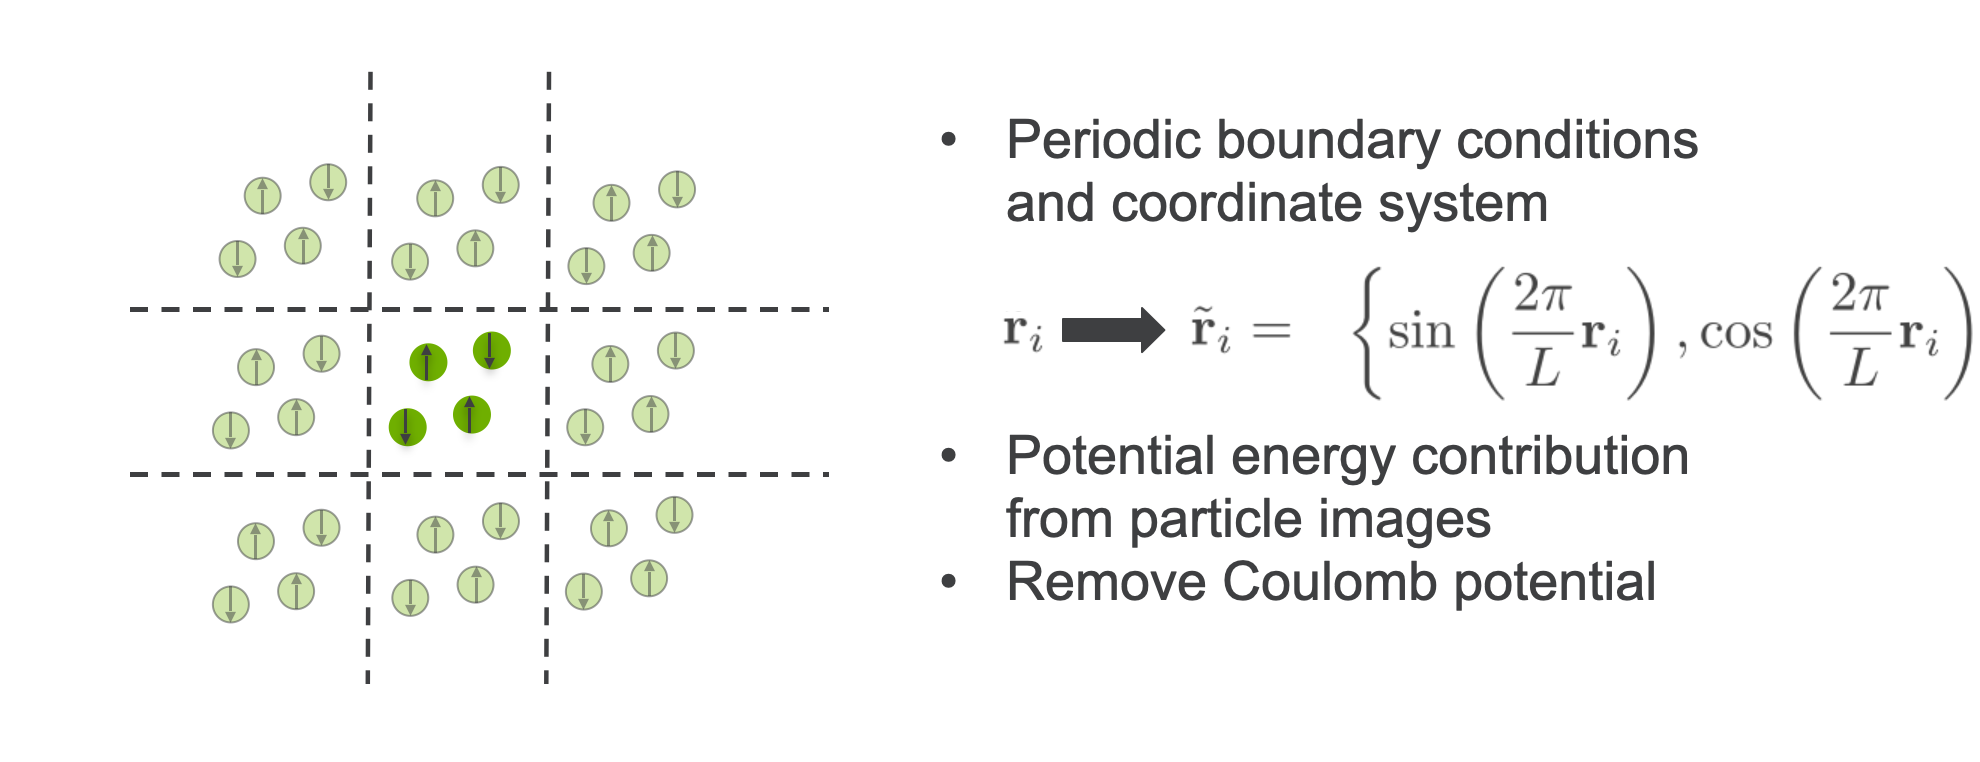
\includegraphics[width=1.0\linewidth]{figures/mbpfig4.png}}

\vspace{6mm}
\end{frame}

\begin{frame}[plain,fragile]
\frametitle{Neutron star structure}

\vspace{6mm}

% inline figure
\centerline{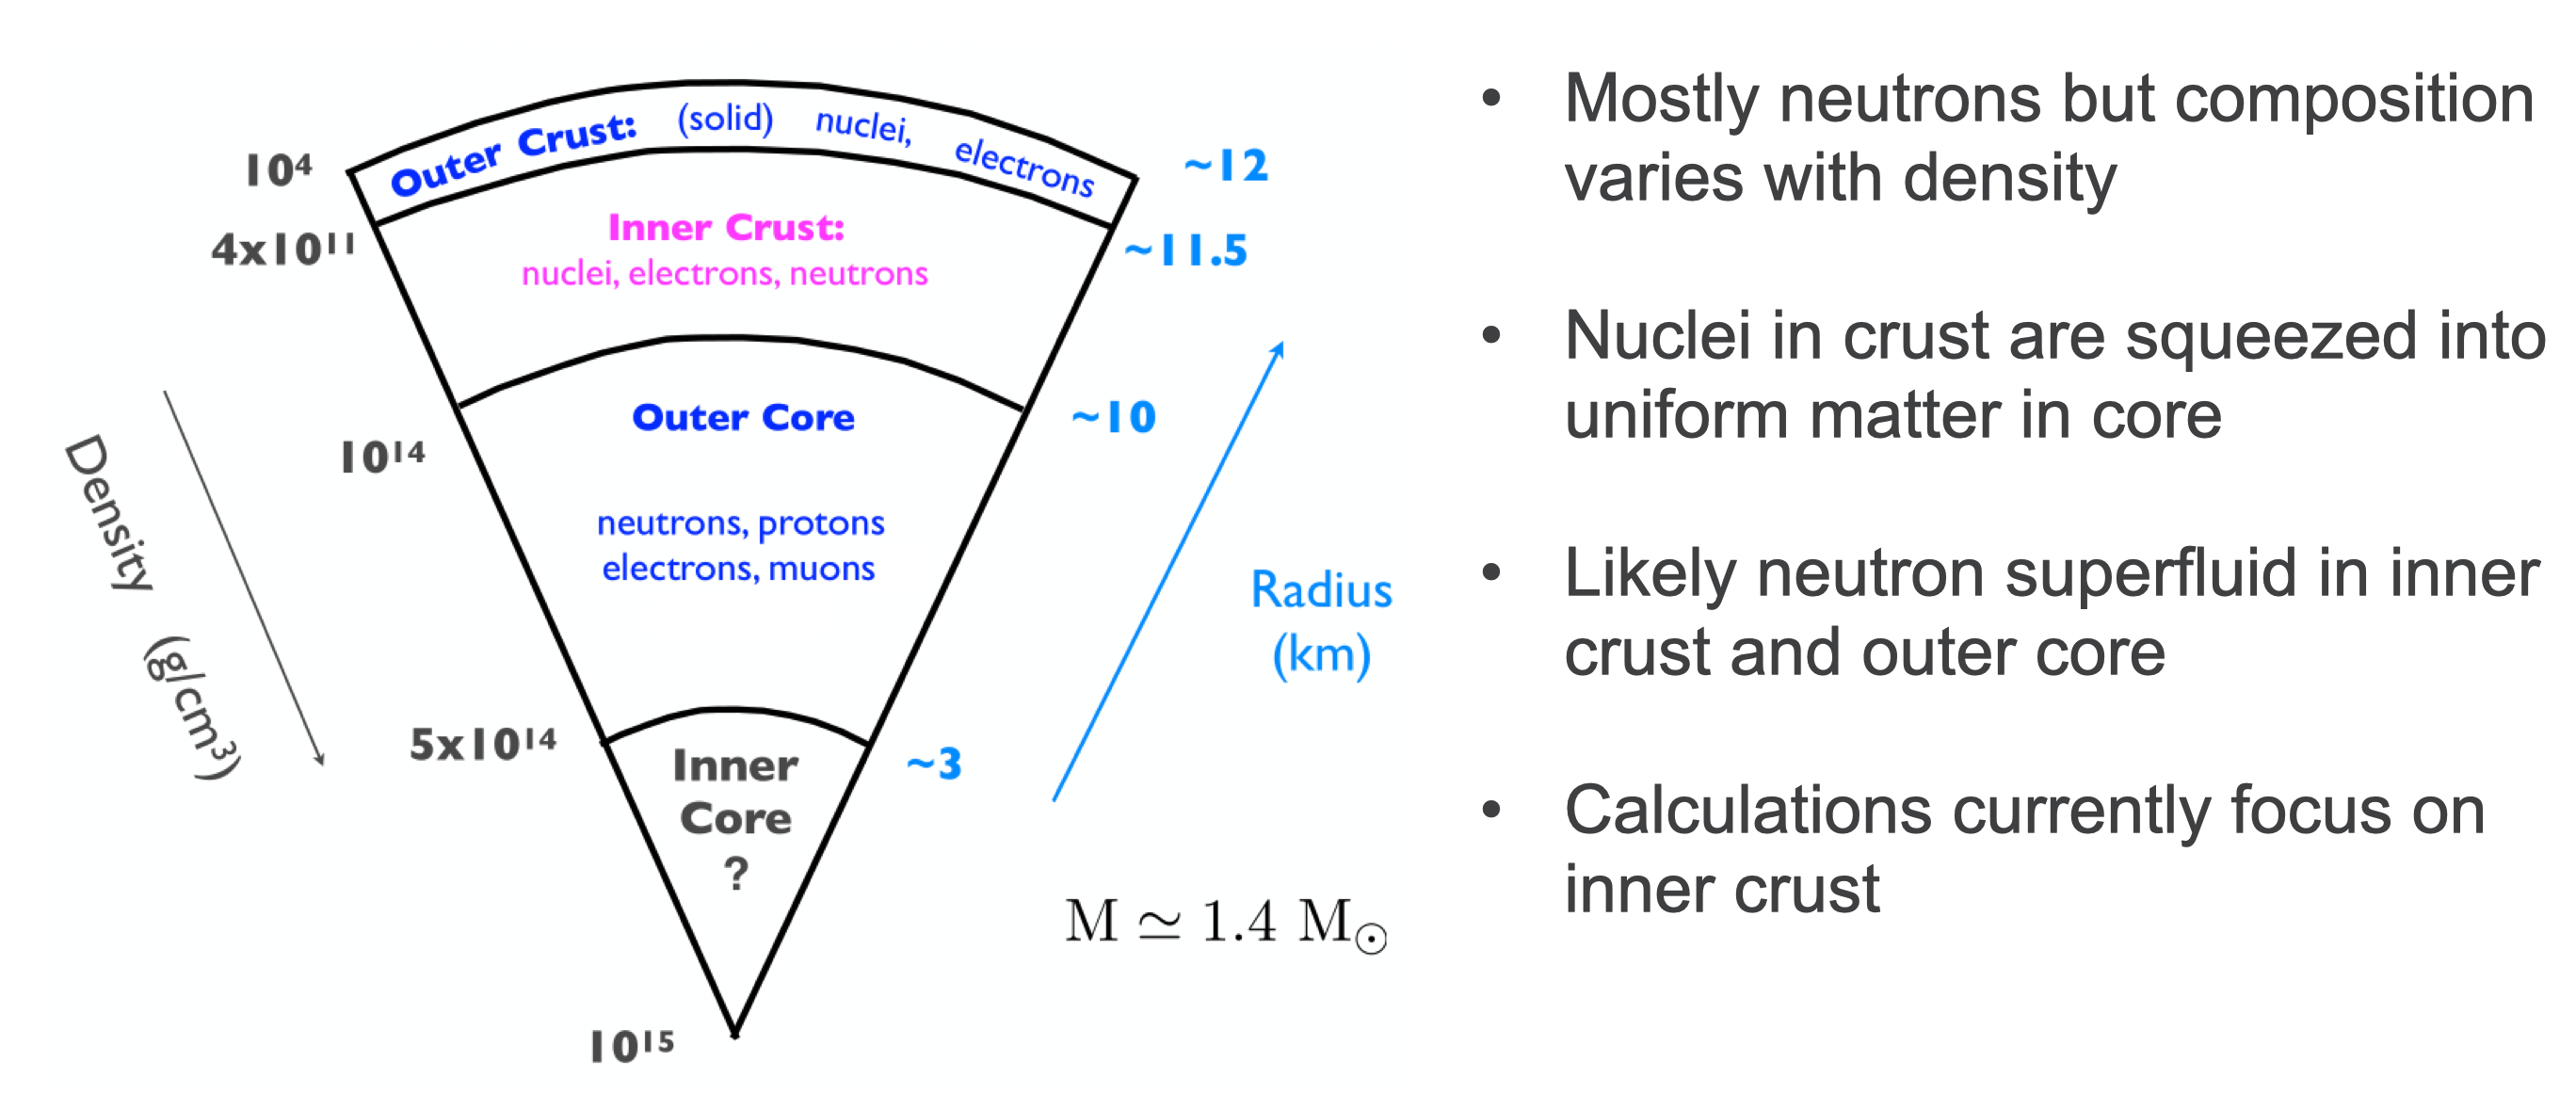
\includegraphics[width=1.0\linewidth]{figures/mbpfig5.png}}

\vspace{6mm}
\end{frame}

\begin{frame}[plain,fragile]
\frametitle{\href{{https://journals.aps.org/prresearch/pdf/10.1103/PhysRevResearch.5.033062}}{Dilute neutron star matter from neural-network quantum states by Fore et al, Physical Review Research 5, 033062 (2023)} at density $\rho=0.04$ fm$^{-3}$}

\begin{block}{}

\vspace{6mm}

% inline figure
\centerline{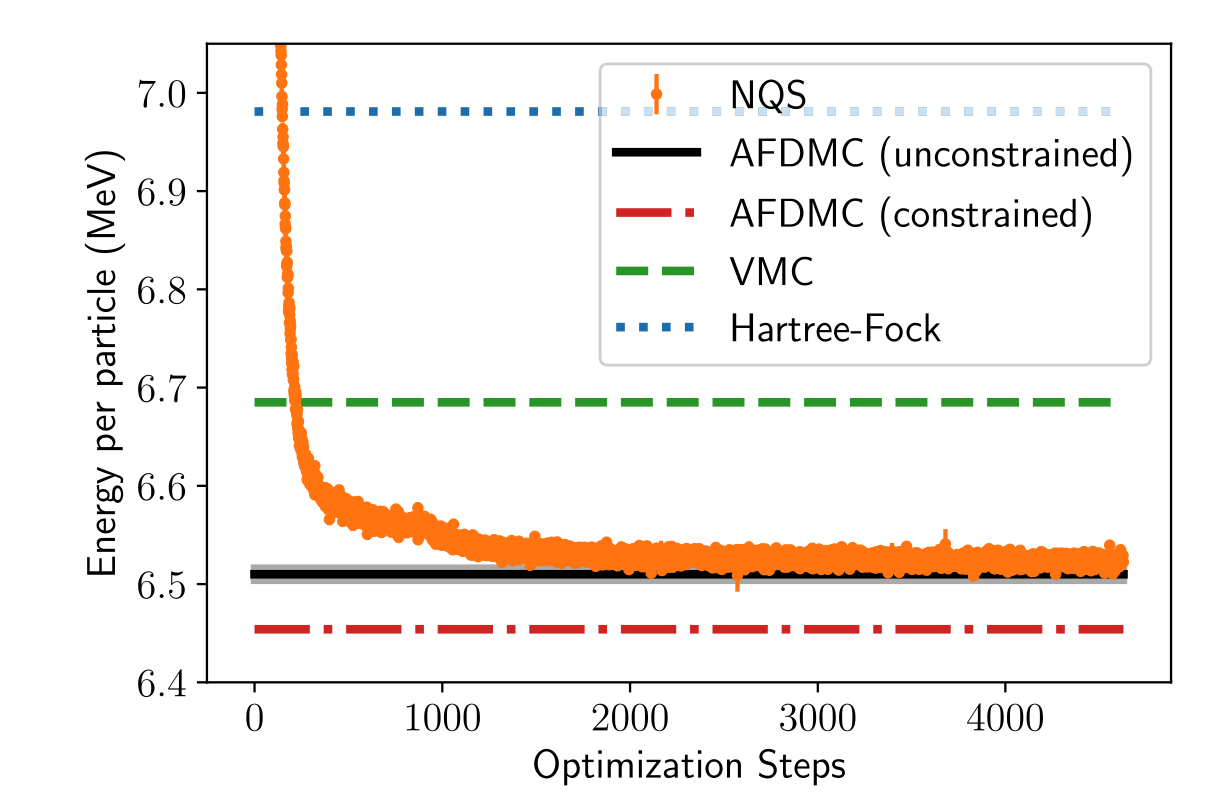
\includegraphics[width=0.9\linewidth]{figures/nmatter.png}}

\vspace{6mm}

\end{block}
\end{frame}

\begin{frame}[plain,fragile]
\frametitle{Pairing and Spin-singlet and triplet two-body distribution functions at $\rho=0.01$ fm$^{-3}$}

\begin{block}{}

\vspace{6mm}

% inline figure
\centerline{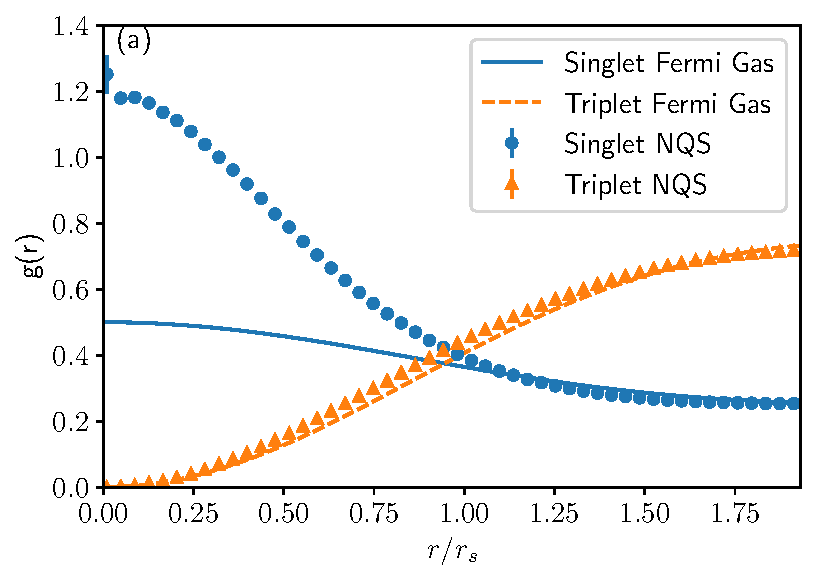
\includegraphics[width=0.9\linewidth]{figures/01_tbd.pdf}}

\vspace{6mm}

\end{block}
\end{frame}

\begin{frame}[plain,fragile]
\frametitle{Pairing and Spin-singlet and triplet two-body distribution functions at $\rho=0.04$ fm$^{-3}$}

\begin{block}{}

\vspace{6mm}

% inline figure
\centerline{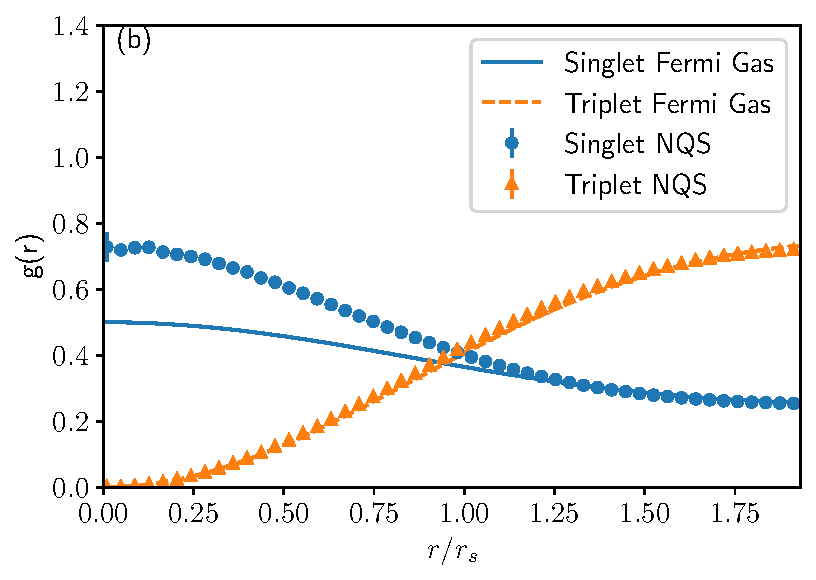
\includegraphics[width=0.9\linewidth]{figures/04_tbd.pdf}}

\vspace{6mm}

\end{block}
\end{frame}

\begin{frame}[plain,fragile]
\frametitle{Pairing and Spin-singlet and triplet two-body distribution functions at $\rho=0.08$ fm$^{-3}$}

\begin{block}{}

\vspace{6mm}

% inline figure
\centerline{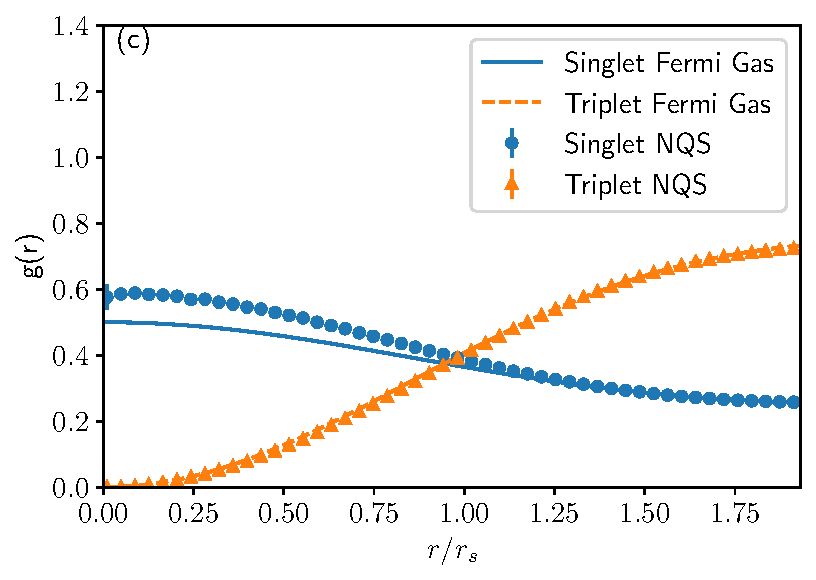
\includegraphics[width=0.9\linewidth]{figures/08_tbd.pdf}}

\vspace{6mm}

\end{block}
\end{frame}

\begin{frame}[plain,fragile]
\frametitle{Symmetric nuclear matter}

\vspace{6mm}

% inline figure
\centerline{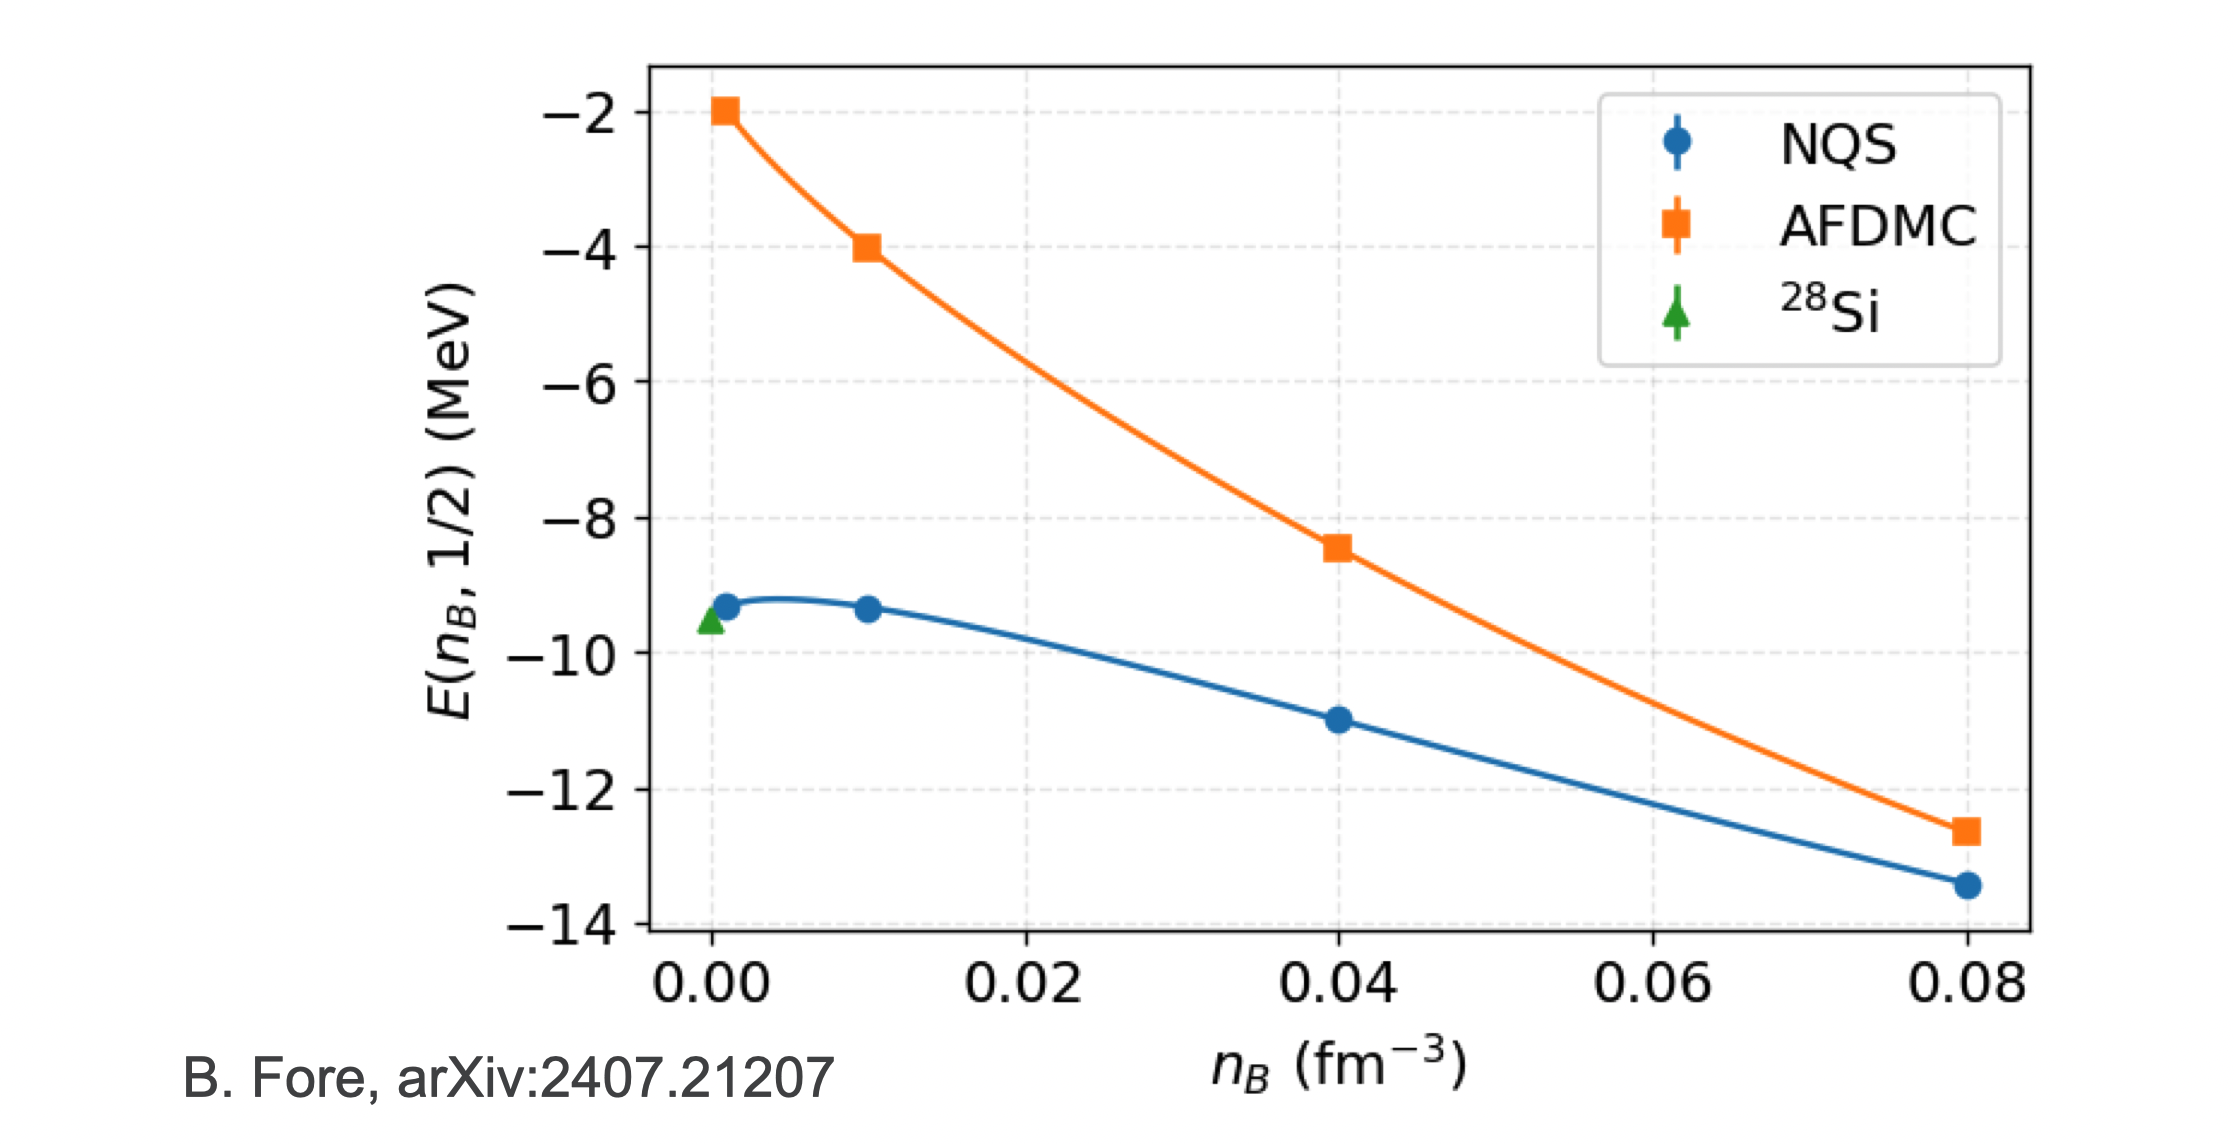
\includegraphics[width=1.0\linewidth]{figures/mbpfig6.png}}

\vspace{6mm}
\end{frame}

\begin{frame}[plain,fragile]
\frametitle{Self-emerging clustering}

\vspace{6mm}

% inline figure
\centerline{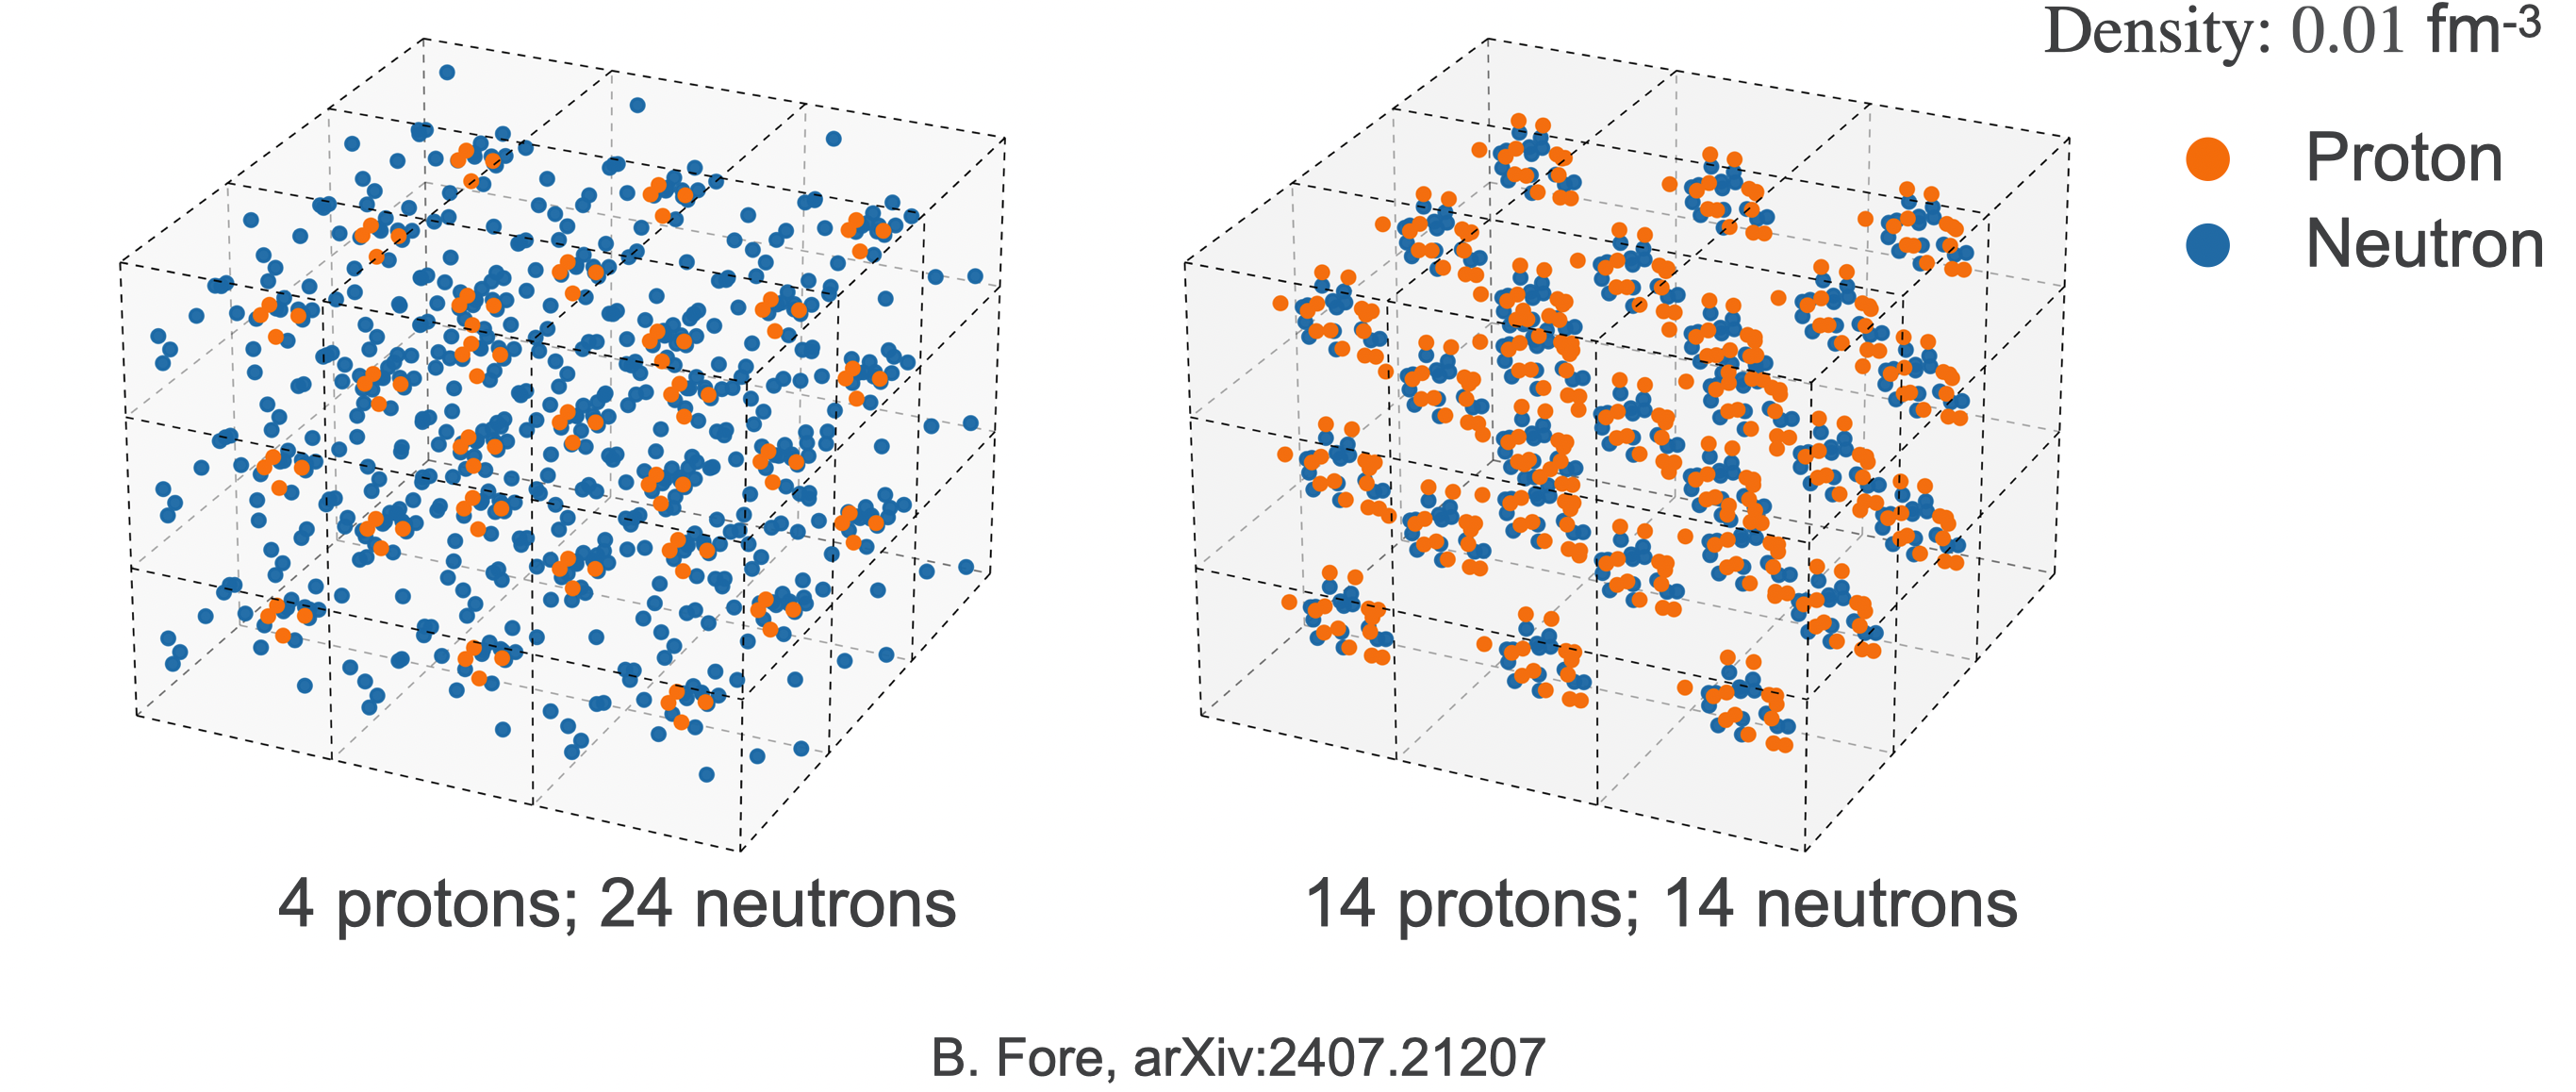
\includegraphics[width=1.0\linewidth]{figures/mbpfig7.png}}

\vspace{6mm}
\end{frame}

\begin{frame}[plain,fragile]
\frametitle{Clustering: Two-body pair distributions}

\vspace{6mm}

% inline figure
\centerline{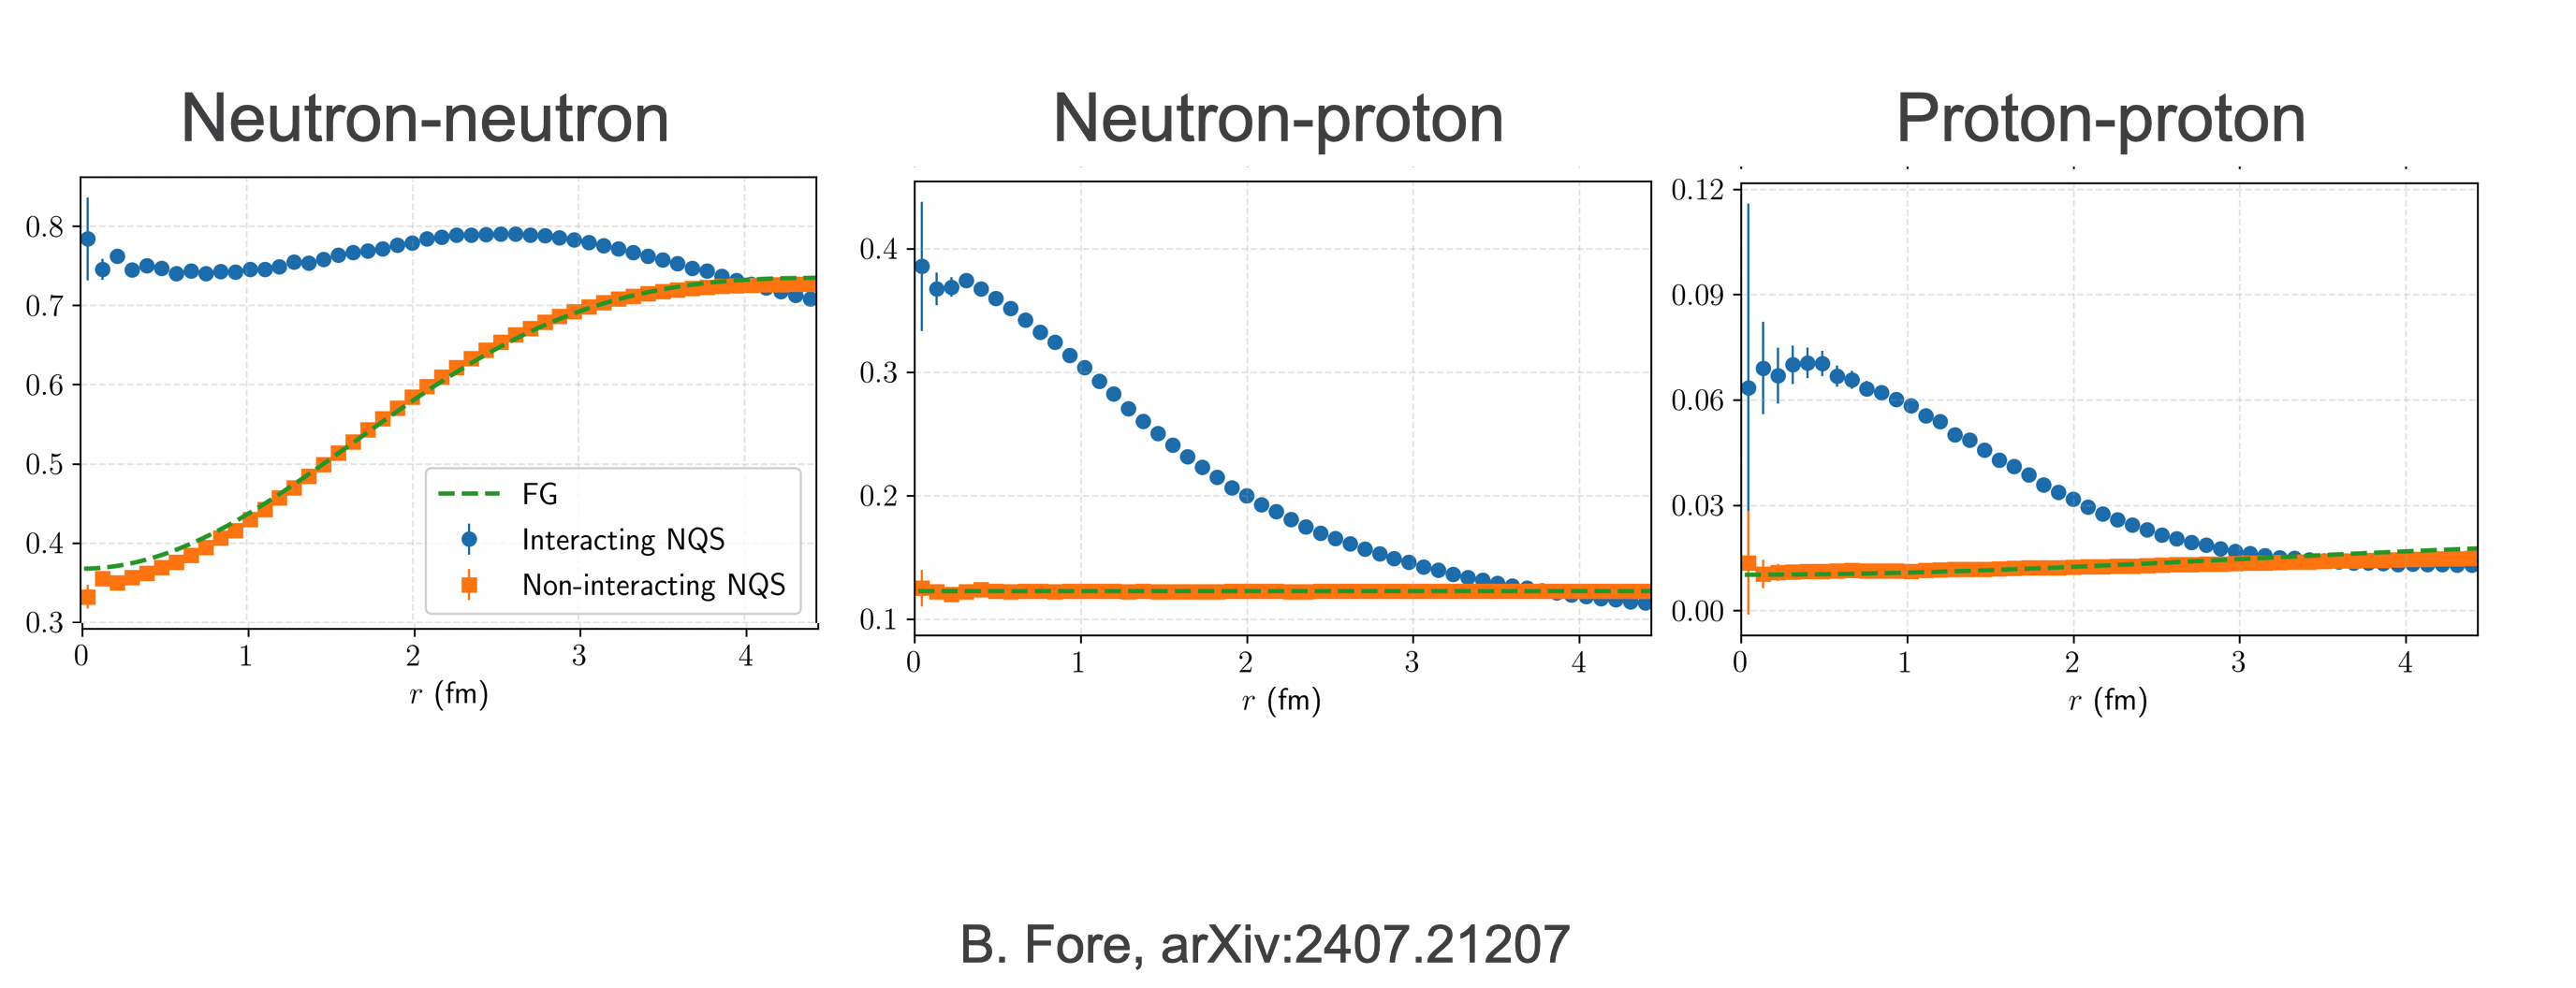
\includegraphics[width=1.0\linewidth]{figures/mbpfig8.png}}

\vspace{6mm}
\end{frame}

\begin{frame}[plain,fragile]
\frametitle{Nuclear matter proton fraction}

\vspace{6mm}

% inline figure
\centerline{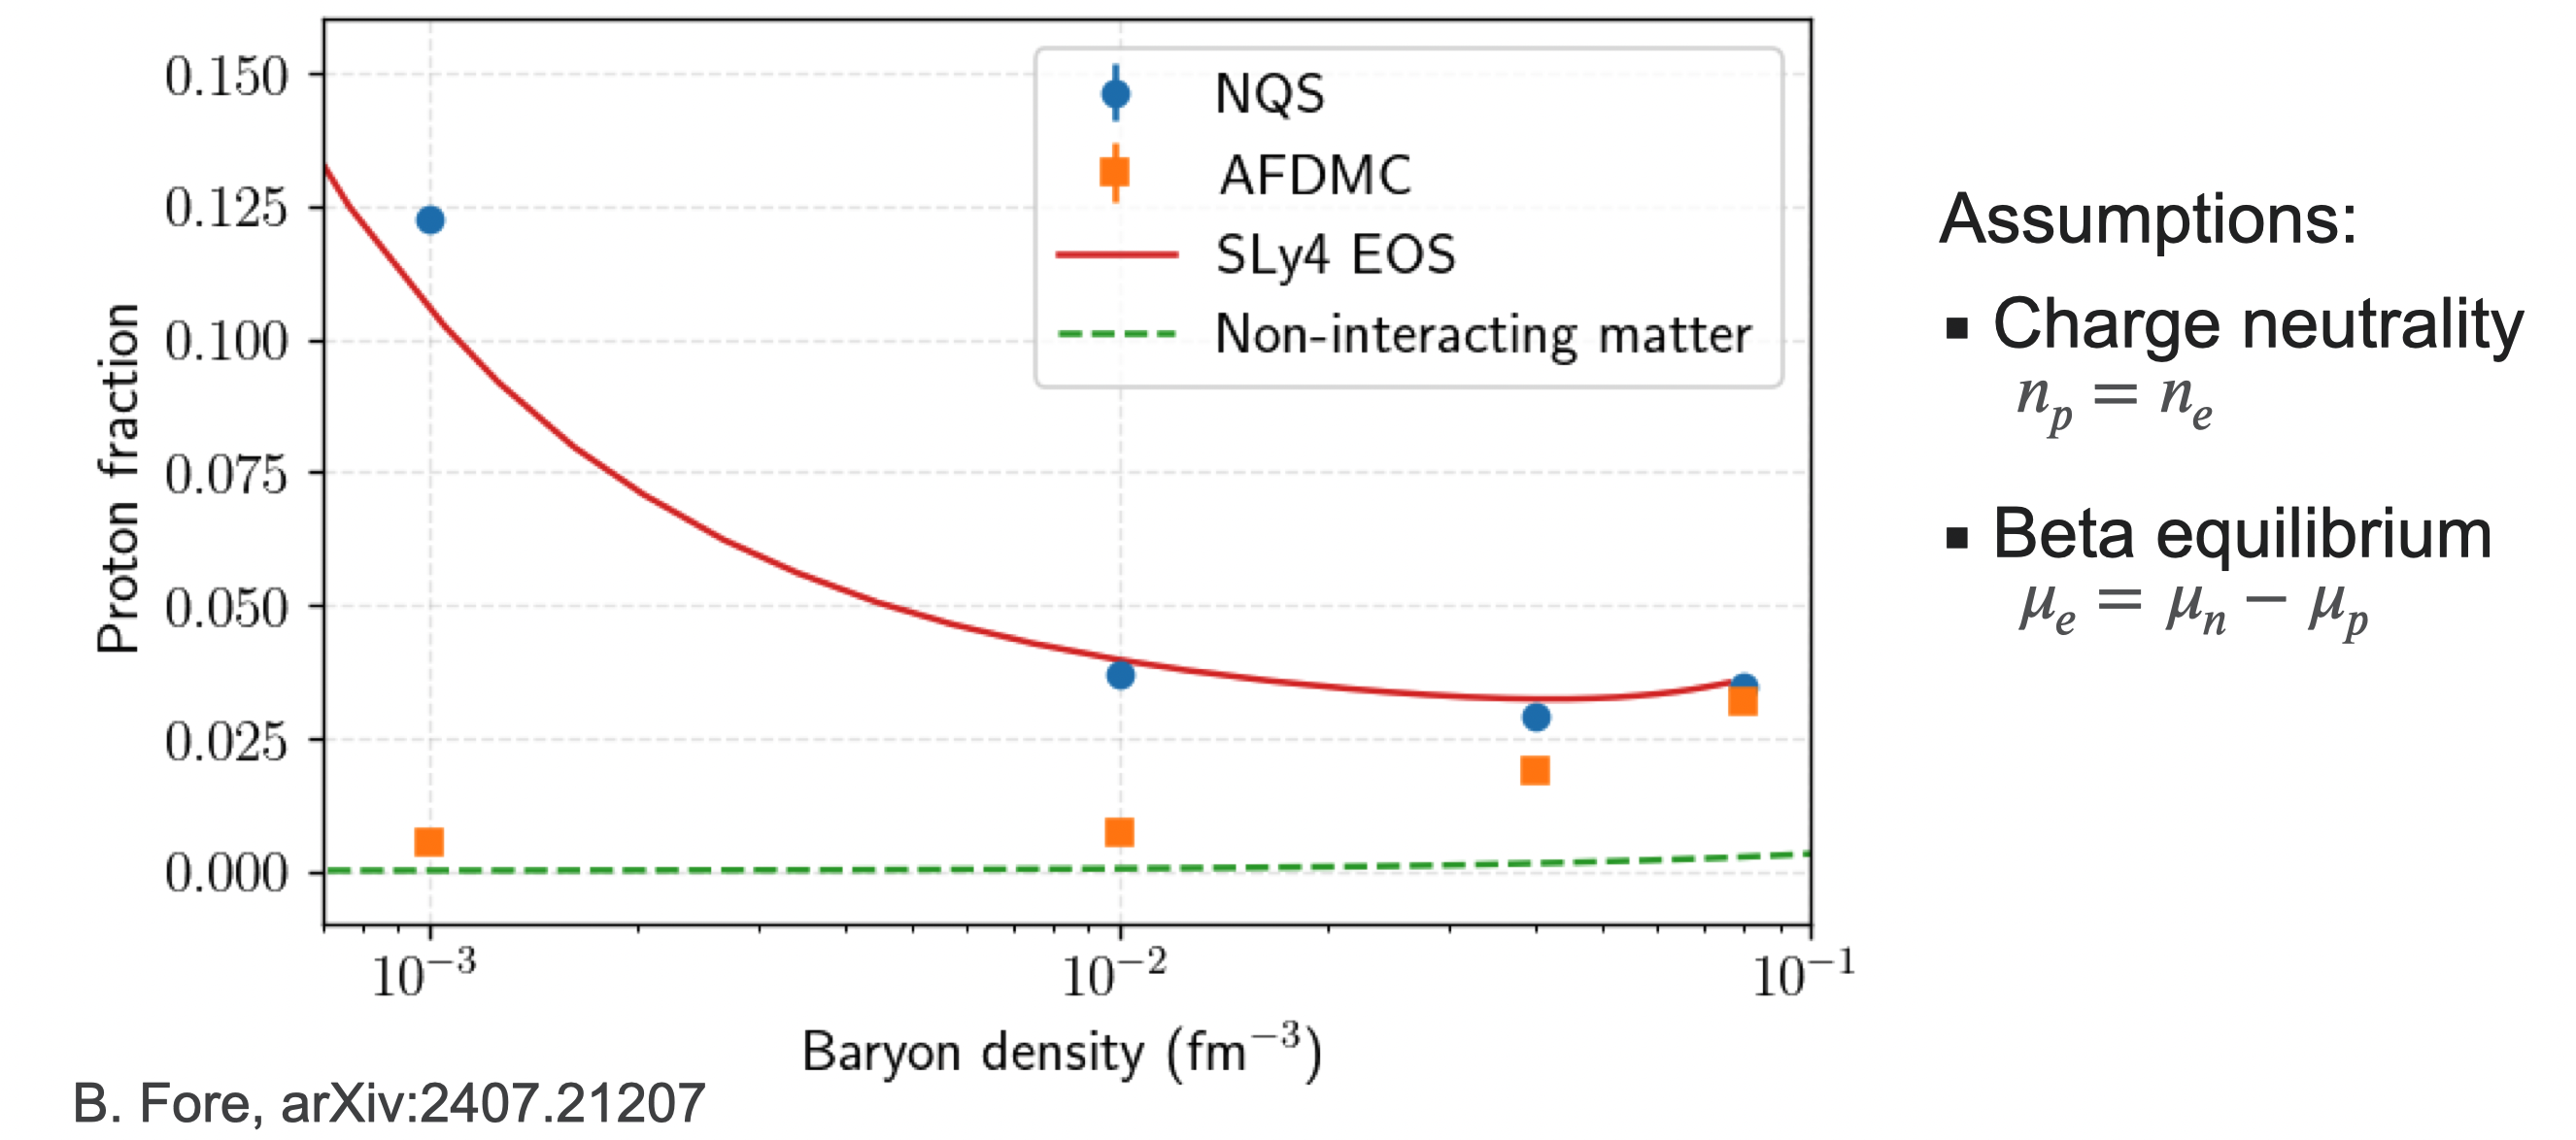
\includegraphics[width=1.0\linewidth]{figures/mbpfig9.png}}

\vspace{6mm}
\end{frame}

\begin{frame}[plain,fragile]
\frametitle{The electron gas in three dimensions with $N=14$ electrons (Wigner-Seitz radius $r_s=2$ a.u.), \href{{https://doi.org/10.48550/arXiv.2305.07240}}{Gabriel Pescia, Jane Kim et al.~arXiv.2305.07240,}}

\begin{block}{}

\vspace{6mm}

% inline figure
\centerline{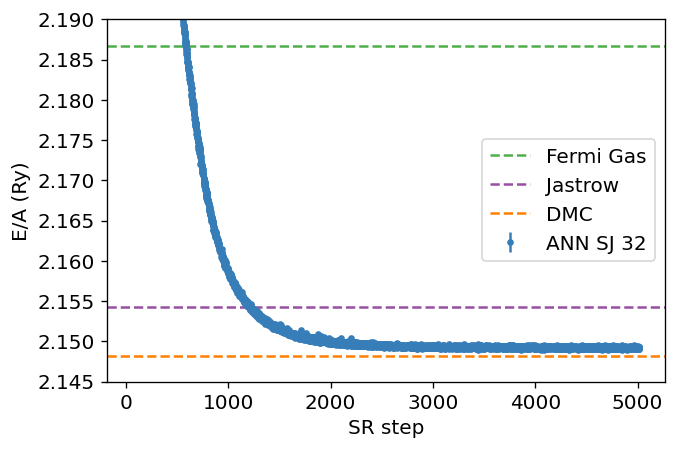
\includegraphics[width=0.9\linewidth]{figures/elgasnew.png}}

\vspace{6mm}

\end{block}
\end{frame}
























































\begin{minted}[fontsize=\fontsize{9pt}{9pt},linenos=false,mathescape,baselinestretch=1.0,fontfamily=tt,xleftmargin=2mm]{python}
# import necessary packages
import numpy as np
import matplotlib.pyplot as plt

def feed_forward(x):
    # weighted sum of inputs to the output layer
    z_1 = x*output_weights + output_bias
    # Output from output node (one node only)
    # Here the output is equal to the input
    a_1 = z_1
    return a_1

def backpropagation(x, y):
    a_1 = feed_forward(x)
    # derivative of cost function
    derivative_cost = a_1 - y
    # the variable delta in the equations, note that output a_1 = z_1, its derivatives wrt z_o is thus 1
    delta_1 = derivative_cost
    # gradients for the output layer
    output_weights_gradient = delta_1*x
    output_bias_gradient = delta_1
    # The cost function is 0.5*(a_1-y)^2. This gives a measure of the error for each iteration
    return output_weights_gradient, output_bias_gradient

# ensure the same random numbers appear every time
np.random.seed(0)
# Input variable
x = 4.0
# Target values
y = 2*x+1.0

# Defining the neural network
n_inputs = 1
n_outputs = 1
# Initialize the network
# weights and bias in the output layer
output_weights = np.random.randn()
output_bias = np.random.randn()

# implementing a simple gradient descent approach with fixed learning rate
eta = 0.01
for i in range(40):
    # calculate gradients from back propagation
    derivative_w1, derivative_b1 = backpropagation(x, y)
    # update weights and biases
    output_weights -= eta * derivative_w1
    output_bias -= eta * derivative_b1
# our final prediction after training
ytilde = output_weights*x+output_bias
print(0.5*((ytilde-y)**2))


\end{minted}

Running this code gives us an acceptable results after some 40-50 iterations. Note that the results depend on the value of the learning rate.
\end{frame}

\begin{frame}[plain,fragile]
\frametitle{Central magic}

\href{{https://en.wikipedia.org/wiki/Automatic_differentiation}}{Automatic differentiation}
\end{frame}

\begin{frame}[plain,fragile]
\frametitle{\href{{https://doi.org/10.3389/fphy.2023.1061580}}{Efficient solutions of fermionic systems using artificial neural networks, Nordhagen et al, Frontiers in Physics 11, 2023}}

The Hamiltonian of the quantum dot is given by
\[ \hat{H} = \hat{H}_0 + \hat{V}, 
\]
where $\hat{H}_0$ is the many-body HO Hamiltonian, and $\hat{V}$ is the
inter-electron Coulomb interactions. In dimensionless units,
\[ \hat{V}= \sum_{i < j}^N \frac{1}{r_{ij}},
\]
with $r_{ij}=\sqrt{\mathbf{r}_i^2 - \mathbf{r}_j^2}$.

Separable Hamiltonian with the relative motion part ($r_{ij}=r$)
\[ 
\hat{H}_r=-\nabla^2_r + \frac{1}{4}\omega^2r^2+ \frac{1}{r},
\]
Analytical solutions in two and three dimensions (\href{{https://journals.aps.org/pra/abstract/10.1103/PhysRevA.48.3561}}{M. Taut 1993 and 1994}).
\end{frame}

\begin{frame}[plain,fragile]
\frametitle{Generative models: Why Boltzmann machines?}

What is known as restricted Boltzmann Machines (RMB) have received a
lot of attention lately.  One of the major reasons is that they can be
stacked layer-wise to build deep neural networks that capture
complicated statistics.

The original RBMs had just one visible layer and a hidden layer, but
recently so-called Gaussian-binary RBMs have gained quite some
popularity in imaging since they are capable of modeling continuous
data that are common to natural images.

Furthermore, they have been used to solve complicated quantum
mechanical many-particle problems or classical statistical physics
problems like the Ising and Potts classes of models.
\end{frame}

\begin{frame}[plain,fragile]
\frametitle{The structure of the RBM network}

\vspace{6mm}

% inline figure
\centerline{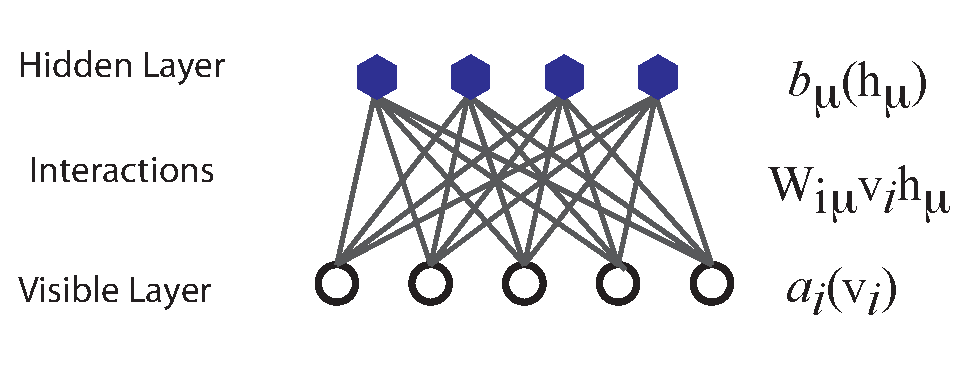
\includegraphics[width=1.0\linewidth]{figures/RBM.pdf}}

\vspace{6mm}
\end{frame}

\begin{frame}[plain,fragile]
\frametitle{The network}

\textbf{The network layers}:
\begin{enumerate}
 \item A function $\bm{x}$ that represents the visible layer, a vector of $M$ elements (nodes). This layer represents both what the RBM might be given as training input, and what we want it to be able to reconstruct. This might for example be the pixels of an image, the spin values of the Ising model, or coefficients representing speech.

 \item The function $\bm{h}$ represents the hidden, or latent, layer. A vector of $N$ elements (nodes). Also called "feature detectors".
\end{enumerate}

\noindent
\end{frame}

\begin{frame}[plain,fragile]
\frametitle{Goals}

The goal of the hidden layer is to increase the model's expressive
power. We encode complex interactions between visible variables by
introducing additional, hidden variables that interact with visible
degrees of freedom in a simple manner, yet still reproduce the complex
correlations between visible degrees in the data once marginalized
over (integrated out).

\textbf{The network parameters, to be optimized/learned}:
\begin{enumerate}
 \item $\bm{a}$ represents the visible bias, a vector of same length as $\bm{x}$.

 \item $\bm{b}$ represents the hidden bias, a vector of same lenght as $\bm{h}$.

 \item $W$ represents the interaction weights, a matrix of size $M\times N$.
\end{enumerate}

\noindent
\end{frame}

\begin{frame}[plain,fragile]
\frametitle{Joint distribution}

The restricted Boltzmann machine is described by a Bolztmann distribution
\[
	P_{\mathrm{rbm}}(\bm{x},\bm{h}) = \frac{1}{Z} \exp{-E(\bm{x},\bm{h})},
\]
where $Z$ is the normalization constant or partition function, defined as 
\[
	Z = \int \int \exp{-E(\bm{x},\bm{h})} d\bm{x} d\bm{h}.
\]
Note the absence of the inverse temperature in these equations.
\end{frame}

\begin{frame}[plain,fragile]
\frametitle{Network Elements, the energy function}

The function $E(\bm{x},\bm{h})$ gives the \textbf{energy} of a
configuration (pair of vectors) $(\bm{x}, \bm{h})$. The lower
the energy of a configuration, the higher the probability of it. This
function also depends on the parameters $\bm{a}$, $\bm{b}$ and
$W$. Thus, when we adjust them during the learning procedure, we are
adjusting the energy function to best fit our problem.
\end{frame}

\begin{frame}[plain,fragile]
\frametitle{Defining different types of RBMs (Energy based models)}

There are different variants of RBMs, and the differences lie in the types of visible and hidden units we choose as well as in the implementation of the energy function $E(\bm{x},\bm{h})$. The connection between the nodes in the two layers is given by the weights $w_{ij}$. 

\begin{block}{Binary-Binary RBM: }

RBMs were first developed using binary units in both the visible and hidden layer. The corresponding energy function is defined as follows:
\[
	E(\bm{x}, \bm{h}) = - \sum_i^M x_i a_i- \sum_j^N b_j h_j - \sum_{i,j}^{M,N} x_i w_{ij} h_j,
\]
where the binary values taken on by the nodes are most commonly 0 and 1.
\end{block}
\end{frame}

\begin{frame}[plain,fragile]
\frametitle{Gaussian binary}

\begin{block}{Gaussian-Binary RBM: }

Another varient is the RBM where the visible units are Gaussian while the hidden units remain binary:
\[
	E(\bm{x}, \bm{h}) = \sum_i^M \frac{(x_i - a_i)^2}{2\sigma_i^2} - \sum_j^N b_j h_j - \sum_{i,j}^{M,N} \frac{x_i w_{ij} h_j}{\sigma_i^2}. 
\]
\end{block}
\end{frame}

\begin{frame}[plain,fragile]
\frametitle{Representing the wave function}

The wavefunction should be a probability amplitude depending on
 $\bm{x}$. The RBM model is given by the joint distribution of
 $\bm{x}$ and $\bm{h}$

\[
        P_{\mathrm{rbm}}(\bm{x},\bm{h}) = \frac{1}{Z} \exp{-E(\bm{x},\bm{h})}.
\]

To find the marginal distribution of $\bm{x}$ we set:

\[
        P_{\mathrm{rbm}}(\bm{x}) =\frac{1}{Z}\sum_{\bm{h}} \exp{-E(\bm{x}, \bm{h})}.
\]

Now this is what we use to represent the wave function, calling it a neural-network quantum state (NQS)
\[
        \vert\Psi (\bm{X})\vert^2 = P_{\mathrm{rbm}}(\bm{x}).
\]
\end{frame}

\begin{frame}[plain,fragile]
\frametitle{Define the cost function}

Now we don't necessarily have training data (unless we generate it by
using some other method). However, what we do have is the variational
principle which allows us to obtain the ground state wave function by
minimizing the expectation value of the energy of a trial wavefunction
(corresponding to the untrained NQS). Similarly to the traditional
variational Monte Carlo method then, it is the local energy we wish to
minimize. The gradient to use for the stochastic gradient descent
procedure is

\[
	C_i = \frac{\partial \langle E_L \rangle}{\partial \theta_i}
	= 2(\langle E_L \frac{1}{\Psi}\frac{\partial \Psi}{\partial \theta_i} \rangle - \langle E_L \rangle \langle \frac{1}{\Psi}\frac{\partial \Psi}{\partial \theta_i} \rangle ),
\]
where the local energy is given by
\[
	E_L = \frac{1}{\Psi} \hat{\bm{H}} \Psi.
\]
\end{frame}

\begin{frame}[plain,fragile]
\frametitle{Quantum dots and Boltzmann machines, onebody densities $N=6$, $\hbar\omega=0.1$ a.u.}

\begin{block}{}

\vspace{6mm}

% inline figure
\centerline{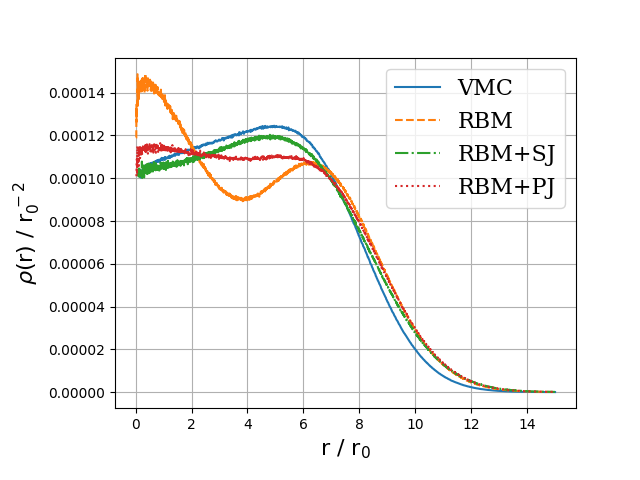
\includegraphics[width=0.9\linewidth]{figures/OB6hw01.png}}

\vspace{6mm}

\end{block}
\end{frame}

\begin{frame}[plain,fragile]
\frametitle{Onebody densities $N=30$, $\hbar\omega=1.0$ a.u.}

\begin{block}{}

\vspace{6mm}

% inline figure
\centerline{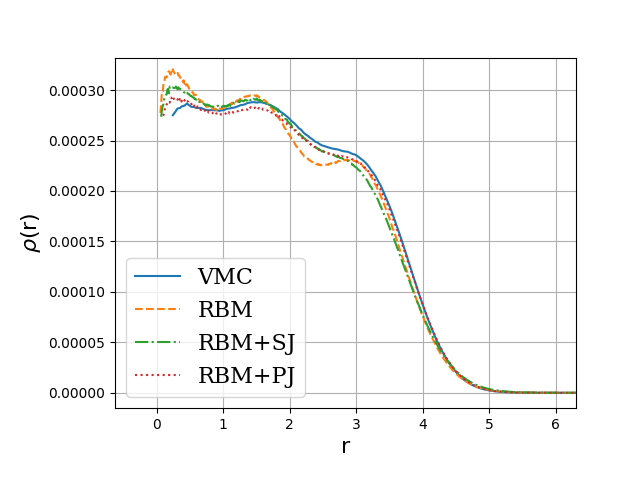
\includegraphics[width=0.9\linewidth]{figures/OB30hw1.png}}

\vspace{6mm}

\end{block}
\end{frame}

\begin{frame}[plain,fragile]
\frametitle{Expectation values as functions of the oscillator frequency}

\begin{block}{}

\vspace{6mm}

% inline figure
\centerline{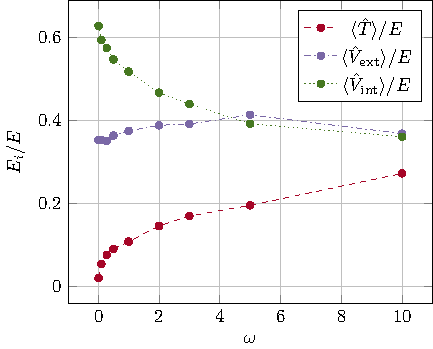
\includegraphics[width=0.9\linewidth]{figures/virialtheorem.pdf}}

\vspace{6mm}

\end{block}
\end{frame}

\end{document}
